\documentclass[10pt,a4paper,oneside]{book}

%Hello there. Don't know what to do?
	%Search for the %? or \fixme and fix/add stuff.
	%Check zapiski 2007, your notes and your memory and fix/add stuff
	%kul knjige imajo quote na začetku poglavij
%
%lol, windows newline bug poje to vrsto na začetku včasih :P
%\documentclass[10pt,a4paper,oneside]{book}

\usepackage[slovene]{babel}
\usepackage[utf8x]{inputenc}
\usepackage[fleqn]{amsmath}%fleqn - levo zamaknjene enačbe
\usepackage{amsfonts}
\usepackage{amssymb}
\usepackage{makeidx}
\usepackage{graphicx}
\usepackage[x11names, rgb]{xcolor}
\usepackage{tikz}
\usetikzlibrary{calc,automata,snakes,arrows,shapes,decorations,positioning,shapes.arrows,chains,shadows}
%\usepackage{nag}

%poglej torstyle.sty
\usepackage{torstyle}

\hypersetup{pdftitle={Teoreticne osnove racunalnistva}}

\begin{document}
\begin{titlepage}
\begin{center}
\ \\[1cm]
{\Huge\bf Teoreti\v cne osnove ra\v cunalni\v stva}\\[1cm]
{\huge \today}\ \\[1.55cm]
%{\LARGE Zapiski predavanj 2010/2011}\\[15pt]%Odkar sem dodal kontekstno-odvisne in linearne, to ni več samo to :P
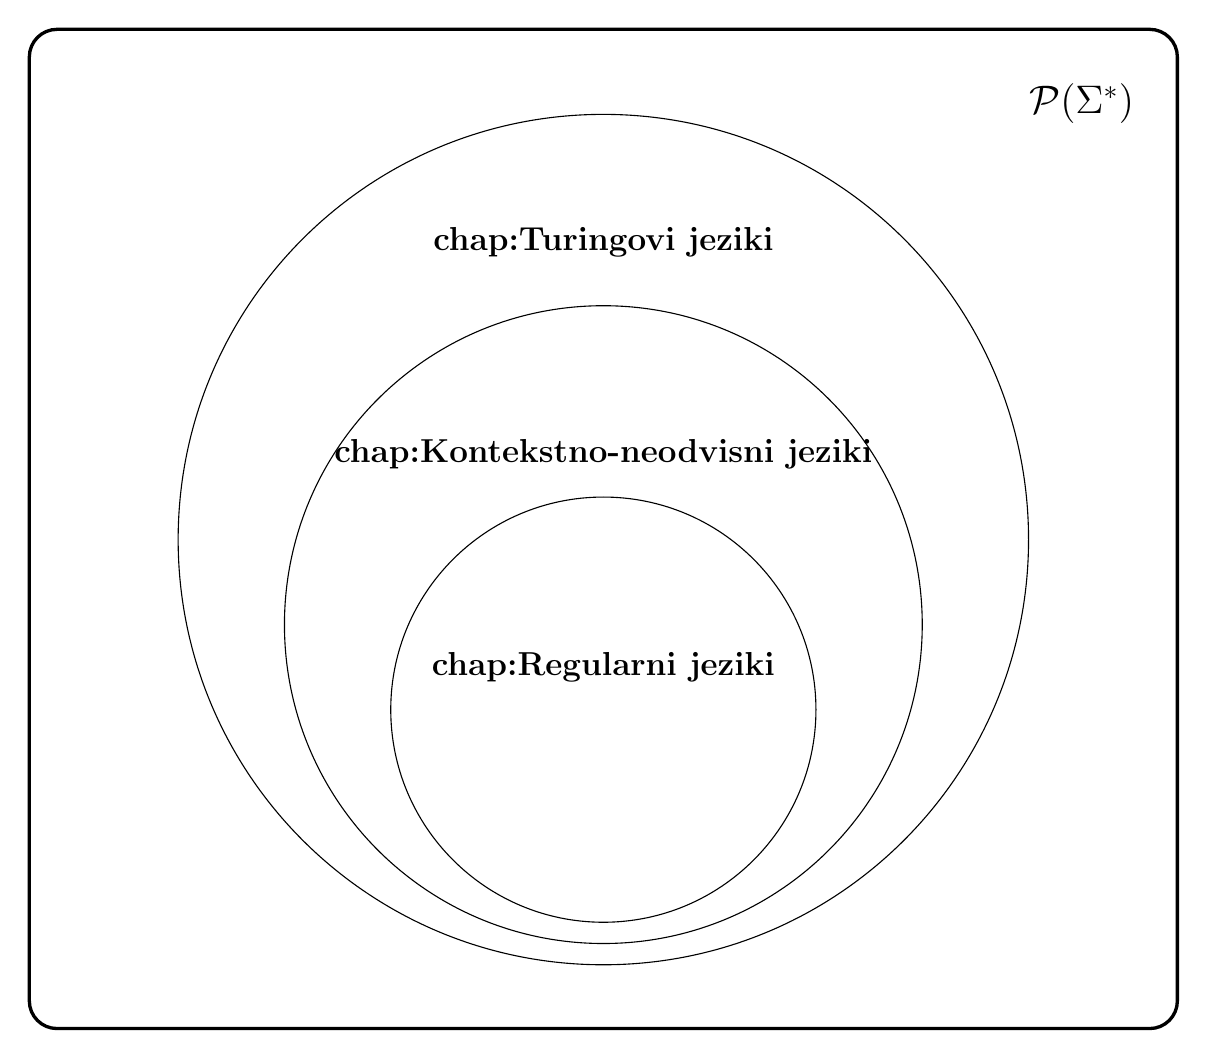
\begin{tikzpicture}[scale=1.35, very thick, circ/.style={thin}]%?tole ful upočasni pdflatex%, decorate, decoration={snake, amplitude=0.75pt}}]
	\draw [rounded corners=10pt] (-5.4cm,-5.4cm) rectangle (5.4cm,4.0cm);
	\node at (4.5cm,3.3cm) {\Large $\mathcal{P}(\Sigma^*)$};%sva šla vprašat... ker \Sigma^* znajo že RJ opisat, samo ne vseh možnih ;)

	%\draw[circ] (0cm,0cm) circle (5cm);
	%\node at (0,4cm) {\large\bf \nameref{chap:Turingovi jeziki}};

	\draw[circ] (0cm,-0.8cm) circle (4cm);
	\node at (0,2cm) {\large\bf \nameref{chap:Turingovi jeziki}};
	%\node at (0,2cm) {\large\bf \nameref{chap:Kontekstno-odvisni jeziki}};

	\draw[circ] (0cm,-1.6cm) circle (3cm);
	\node at (0,0cm) {\large\bf \nameref{chap:Kontekstno-neodvisni jeziki}};

	\draw[circ] (0cm,-2.4cm) circle (2cm);
	\node at (0,-2cm) {\large\bf \nameref{chap:Regularni jeziki}};
\end{tikzpicture}

\vfill
\parbox{7.5cm}{
\begin{center}

\includegraphics[width=0.15\textwidth]{./by-nc-sa}\\[6pt]

This work is licensed under a Creative Commons Attribution-NonCommercial-ShareAlike 3.0 Unported License
\end{center}
}

\end{center}
\end{titlepage}
\tableofcontents
\pagebreak

%--------------------------------TOR1--------------------------------------

\chap{Uvod}
%\sect{Matematične osnove}
%\newpage
%\sect{Notacija}
%\begin{itemize}
%	\item[Množice:] Označimo z velikimi tiskanimi črkami. Podamo jih lahko na naslednje načine\\
%	$ A = \{ a_1, a_1, a_3, \ldots \} $ - naštevanje elementov\\
%	$ B = \{ n | \ \mbox{pravilo za n} \} \ $ - opis elementov
%\end{itemize}

%?appendix this:
%\chapter{Slovar}
%?zihr obstaja neki za to, sicer naredi definitions okolje
%\begin{items}
%\item Razred - razred je množica elementov, ki ga lahko podamo z naštevanjem elementov ali z opisom lastnosti (opisni ali konceptualni razredi)
%\end{items}

\sect{Osnove dokazovanja}
\subsect{Dokaz s konstrukcijo}
Dokaz obstoja nekega matematičnega objekta je to, da nam ga uspe sestaviti.

\begin{primeri}
\item Za vsak $n>4$, obstaja dvojiško drevo, ki ima natanko $3$ liste.\\
	Primer za $n=5$:
	\br
	\hspace*{1cm}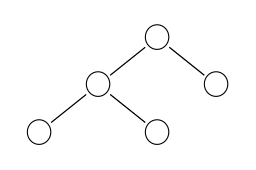
\begin{tikzpicture}[level distance=6mm, inner sep=-0.3mm]
		\node (root) {$\bigcirc$}
		child { node (a) {$\bigcirc$} 
			child { node (b) {$\bigcirc$} }
			child { node (c) {$\bigcirc$} }
		}
		child { node (d) {$\bigcirc$} };
	\end{tikzpicture}
	\br
	Primer za $n>5$, pri čemer je "$...$", poljubno vejitev samo v levo:
	\br
	\hspace*{1cm}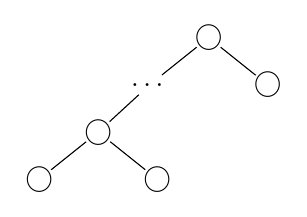
\begin{tikzpicture}[level distance=6mm, inner sep=-0.3mm]
		\node (root) {$\bigcirc$}
		child { node (a) [inner sep=1mm] {$\dots$} {
			child { node (b) [left=0.5cm] {$\bigcirc$} 
				child { node (c) {$\bigcirc$} }
				child { node (d) {$\bigcirc$} }}
		}}
		child { node (e) {$\bigcirc$} };
	\end{tikzpicture}
	\\
\item $| \mathbb{R} | = | [0,1) |$.\\
	\begin{items}
	\item Množici imata enako moč, kadar med njima obstaja bijektivna preslikava.
	\item Vsako realno število $r$ lahko zapišemo kot:
	\[ r=\pm d_1 d_2 \cdots d_n . \overline{d_1}\overline{d_2} \cdots \overline{d_m} \cdots;\ d_1 \neq 0 \]
	\item Definiramo preslikavo:
	\[ \mathbb{R}\rightarrow [0,1): r \rightarrow 0.s\overline{d_1} d_{n} \overline{d_2} d_{n-1} \cdots \overline{d_{n-1}} d_2 \overline{d_n} d_1 \overline{d_{n+1}} 0\overline{d_{n+2}} 0 \cdots \]
	kjer $s$ določa predznak ($s=0$, če $r \ge 0$ in $s=1$, sicer).
	\item Vidimo:
		\begin{items}
		\item $|\mathbb{R}|\ge |[0,1)|$, ker velja $[0,1) \subset \mathbb{R}$
		\item $|\mathbb{R}|\le |[0,1)|$,\fixme%?(ker se $0.2$ ne da preslikati v $\mathbb{R}$)??
		\end{items}
	\item Iz tega lahko sklepamo, da velja $|\mathbb{R}|=|[0,1)|$
	\end{items}
\end{primeri}
	
\subsect{Dokaz z indukcijo}
Če je množica induktivni razred%\footnote{Glej slovarček na koncu.}
, lahko z matematično indukcijo dokazujemo neko lastnost članov množice. Induktivni razred $I$ sestavlja:
\begin{items}
\item Baza indukcije - najbolj osnovna množica elementov (osnovni razred)
\item Pravila generiranja - kako iz elementov baze gradimo nove elemente (množico)
\end{items}
\begin{primeri}
\item Induktivni razred naravnih števil $(\mathbb{N})$
	\begin{items}
	\item Baza: $1 \in \mathbb{N}$ 
	\item Pravila generiranja: $n \in \mathbb{N} \Longrightarrow n+1 \in \mathbb{N} $
	\end{items}
\item Hilbertove krivulje \fixme
\end{primeri}

\subsect{Dokaz s protislovjem}
Vzamemo nasprotno trditev, od tiste, ki jo želimo preveriti in pokažemo, da to vodi v protislovje.

\begin{primeri}
\item Praštevil je končno mnogo.
	\begin{items}
	\item Predpostavimo, da poznamo vsa praštevila:\\
		$P = \{2,3,5,...,p\}$, kjer je $p$ zadnje praštevilo 
	\item Po definiciji obstajajo le praštevila in sestavljena števila (to so taka, ki jih lahko razstavimo na prafaktorje). 
	\item Če pomnožimo vsa znana praštevila iz $P$ in prištejemo $1$ dobimo število, ki se ga ne da razstaviti na prafaktorje iz množice $P$:\\
		$q = 2 * 3 * 5 * ... * p + 1$
	\item Torej je $q$ ali praštevilo (ker ni sestavljeno), ali pa število, sestavljeno iz prafaktorjev, ki jih ni v množici $P$.
	\item Oboje kaže na to, da v množici $P$ nimamo vseh praštevil, ter, da to velja za vsako končno množico praštevil.
	\end{items}
\item $\sqrt[3]{2}$ je racionalno število.
	\begin{items}
	\item Če je $\sqrt[3]{2}$ racionalno število, ga je moč zapisati kot ulomek $\frac{a}{b}$.
	\item Predpostavimo, da je ulomek $\frac{a}{b}$ okrajšan (torej, da velja: $GCD(a,b)=1$):
		\begin{align*}
		\sqrt[3]{2} &= \frac{a}{b}\\
		2 &= \left( \frac{a}{b} \right)^3\\
		2b^3 &= a^3
		\end{align*}
	\item Opazimo, da je $a$ sodo število, torej lahko pišemo $a = 2k$:
		\begin{align*}
		2b &= \left( 2k\right)^3\\
		2b &= 8k\\
		b &= 4k
		\end{align*}
	\item Ker se je pokazalo, da je tudi $b$ sodo število, $GCD(a,b)=1$ ne more držati, torej smo prišli v protislovje in s tem dokazali, da $\sqrt[3]{2}$ ni racionalno število.
	\end{items}
\end{primeri}
\sect{Osnove teorije jezikov}
\subsect{Uporabljene oznake}
\begin{items}
\item $a$ - znak ali simbol
\item $\Sigma$ - abeceda (končna neprazna množica znakov)
\item $w$ - niz ali beseda (poljubno končno zaporedje znakov, $w=a_1a_2 \ldots a_n$)
\item $|w|$ - dolžina niza
\item $\varepsilon$ - prazen niz, $|w|=0$
\item $\Sigma^*$ - vsi nizi nad abecededo
\end{items}

\subsect{Operacije nad jeziki}
\subsubsect{Stik nizov}
	\begin{align*}
	w  &= a_1 a_2 \dots a_n\\
	x  &= b_1 b_2 \dots b_m\\
	wx &= a_1 a_2 \dots a_n b_1 b_2 \dots b_m
	\end{align*}
\subsubsect{Stik množic}
	\begin{align*} 
	A & = \{ w_1 ,\ w_2 ,\ \dots ,\ w_n \} \\ 
	B & = \{ x_1 ,\ x_2 ,\ \dots ,\ x_m \} \\ 
	A \cdot B & = \{ w_ix_j \ | \ w_i \in A \ \wedge \ x_i \in B \}
	\end{align*} 
\subsubsect{Potenciranje}
	\begin{align*} 
	A^0 & = \{ \varepsilon \} \\
	A^k & = A \cdot A \cdot \ldots \cdot A \ = \ \bigcirc_{i=1}^{k} A \\
	\end{align*}
\subsubsect{Iteracija}
	\begin{align*} 
	A^* &= A^0 \cup A^1 \cup A^2 \cdots  \ = \ \bigcup_{i=0}^{ \infty } A^i
	\end{align*} 		
\subsubsect{Obrat}
	\begin{align*}
	\ w\  &= a_1 a_2 \dots a_{n-1} a_n\\
	w^R  &= a_n a_{n-1} \dots a_2 a_1\\
	\end{align*}

\chap{Regularni jeziki}
\sect{Regularni izrazi}\label{sec:RI}
\Def{Imamo tri osnovne izraze:
	\begin{items}
	\item $\underline{\emptyset}$ je opisuje prazen jezik $ L(\underline{\emptyset})= \{ \}$
	\item $\underline{ \varepsilon }$ opisuje jezik $L(\underline{ \varepsilon })= \{ \varepsilon\}$
	\item $\underline{a}$ opisuje jezik $L( \underline{a} ) = \{ a \},\ a \in \Sigma$
	\end{items}
	In tri pravila za generiranje sestavljenih izrazov:
	\begin{items}
	\item $(r_1 + r_2)$ opisuje unijo jezikov $L(r_1 + r_2) = L(r_1) \bigcup L( r_2)$
	\item $(r_1\ r_2)$ opisuje stik jezikov $L(r_1\ r_2) = L(r_1)\cdot L( r_2)$
	\item $(r^*)$ opisuje iteracijo jezika $(L(r))^*$
	\end{items}
}
\begin{primeri}
\item Opiši vse nize, ki se končajo z nizom $00$ v abecedi $\Sigma = \{ 0,1 \}$.
	\[ r = (0+1)^*00 \]
	\item Opiši vse nize, pri katerih so vsi $a$-ji pred $b$-ji in vsi $b$-ji pred $c$-ji v abecedi $\Sigma = \{ a,b,c \}$.
		\[ a^*b^*c^* \]
	\item Opiši vse nize, ki vsebujejo vsaj dva niza '$aa$', ki se ne prekrivata v abecedi $\Sigma = \{ a,b,c \}$.
		\[ (a+b+c)^* aa (a+b+c)^* aa (a+b+c)^* \]
	\item Opiši vse nize, ki vsebuje vsaj dva niza '$aa$' ki se lahko prekrivata v abecedi $\Sigma = \{ a,b,c \}$
		\[ (a+b+c)^* aa (a+b+c)^* aa (a+b+c)^* + (a+b+c)^* aaa (a+b+c)^* \]
	\item Opiši vse nize, ki ne vsebujejo niza $11$ v abecedi $\Sigma = \{ 0,1 \}$
		\[ (\varepsilon  + 1 )(0^*01)^* 0^*	\]
		\[ (\varepsilon  + 1 )(0^* + 01)^* \]
	\item S slovensko abecedo opiši besedo "Ljubljana" v vseh sklonih in vseh mešanicah velikih in malih črk.
		\[ (L+l)(J+j)(U+u)(B+b)(L+l)(J+j)(A+a)(N+n)( (A+a)(O+o)(E+e)(I+i) ) \]
		Koliko različnih nizov opišemo s tem regularnim izrazom?\\
		\[ 2^8 \cdot 2^3 = 2^{11} \mbox{ nizov} \]
\end{primeri}
\sect{Končni avtomati}\label{sec:KA}
\subsect{Nedeterministični končni avtomati z $\varepsilon$-prehodi }
\Def{$\varepsilon$NKA je definiran kot peterka $M = \langle Q, \Sigma, \delta ,q_0 , F \rangle$, kjer je:
	\begin{items}
	\item $ Q $ - končna množica stanj
	\item $ \Sigma $ - vhodna abeceda
	\item $ \delta $ - funkcija prehodov, $\delta : Q \times (\Sigma \cup \{\varepsilon\}) \rightarrow 2^Q$
	\item $ q_0 $ - začetno stanje
	\item $ F $ - množica končnih stanj
	\end{items}
}
%?razlaga potenčne množice bi šla lahko nekam med mat. osnove... imam še en kup stvari o teoriji množic nekje. Drugač je pa kul - epsilon-closure je že napol opisan :)
$2^Q=P(Q)$ je tu potenčna množica stanj avtomata. To pomeni da je so v $2^Q$ vse možne kombinacije stanj. Recimo da se nahajamo v stanju A, potem nas funkcija prehodov $ \delta $ pripelje v vsa mozna stanja do katerih pridemo iz $A$ z določenim znakom abecede in z vsemi $ \varepsilon $ prehodi, naprimer $ \{ A_1,A2, \ldots , A_n \}$. Tukaj je množica stanj $ \{ A_1,A2, \ldots , A_n \} $ element potenčne množice $P(Q)$

\subsect{Nedeterministični končni avtomati}
\Def{NKA je definiran kot peterka $M = \langle Q, \Sigma, \delta, q_0, F \rangle$, kjer je:
	\begin{items}
	\item $ Q $ - končna množica stanj
	\item $ \Sigma $ - vhodna abeceda
	\item $ \delta $ - funkcija prehodov $\delta : Q \times \Sigma \rightarrow 2^{Q}$
	\item $ q_0 $ - začetno stanje
	\item $ F $ - množica končnih stanj
	\end{items}		
}
\Def{Funkcija $\varepsilon$-closure($q$) nam pove, do katerih stanj lahko pridemo iz stanja $q$ po $\varepsilon$ prehodih.
	\[ \varepsilon\mbox{-closure}(q) = \{ q_k\ |\ \exists q_1, q_2, \dots q_n \in Q,\ q=q_1 \wedge q_i \in \delta(q_{i-1}, \varepsilon) \} \]
}
\Def{Posplošena funkcija prehodov $\hat\delta$ nam pove, do katerih stanj pridemo po nekem nizu.		\[ \hat\delta(q, \varepsilon) = \varepsilon\mbox{-closure}(q) \]
	\[ \hat\delta(q, a) = \delta(q, a) \]
	\[ \hat\delta(q, wa) = \varepsilon\mbox{-closure}(\{ q''\ |\ q' \in \hat\delta(q, w) \wedge q'' \in \delta(q', a) \})\]
}

\subsect{Deterministični končni avtomat}
\Def{DKA je definiran kot petorka $M = \langle Q, \Sigma, \delta, q_0, F \rangle$, kjer je:
	\begin{items}
	\item $ Q $ - končna množica stanj
	\item $ \Sigma $ - vhodna abeceda
	\item $ \delta $ - funkcija prehodov, $\delta : Q \times \Sigma \rightarrow Q$
	\item $ q_0 $ - začetno stanje
	\item $ F $ - množica končnih stanj
	\end{items}	
}

\subsect{Jeziki končnih avtomatov}
\Def{Jezik $\varepsilon$NKA ter NKA je definiran kot:
	\begin{equation*}
	L=\{ w\ |\ \hat\delta(q_0, w) \cap F \neq \emptyset \}
	\end{equation*}
	kjer je $\hat\delta(q,w)$ posplošena funkcija prehodov v večih korakih.}
\Def{Jezik DKA je definiran kot:
	\begin{equation*}
	L=\{ w\ |\ \hat\delta(q_0, w) \in F \}
	\end{equation*}
}
Definicije želijo povedati, da so v jeziku točno tisti nizi, po katerih je iz začetnega stanja mogoče priti do nekega končnega stanja.

\sect{Levo in desno-linearne gramatike}\label{sec:LLGDLG}
Posebnost linearnih gramatik je v tem, da imajo na desni strani produkcij največ en vmesni simbol, ampak ta model je že nekoliko močnejši od regularnih jezikov (glej \ref{sec:LG}), če pa se omejimo le na tiste produkcije, ki imajo ta edini vmesni simbol vedno na skrajno levi strani, ali pa vedno na skrajni desni strani niza, dobimo model, ki opisuje regularne jezike.
%
\Def{Linearna gramatika je definirana kot četvorček $G=\langle N,T,P,S \rangle$, kjer je:
\begin{items}
\item N - množica spremenljivk oz. vmesnih simbolov, $N \subseteq \Sigma$
\item T - množica znakov oz. končnih simbolov, $T \subset \Sigma,\ N\cap T = \emptyset$
\item P - množica produkcij
\item S - začetni simbol, $S \in N$
\end{items}
Pri tem je abeceda $\Sigma = N \cup T$ in $N\cap T = \emptyset$.
}
\subsect{Produkcije}
\Def{Pri levo in desno-linearnih gramatikah, s produkcijami slikamo nek vmesni simbol v niz, ki ima lahko vmesni simbol le na skrajno levi pri levo-linearnih, oz. le na skrajno desni pri desno-linearnih:
	\begin{items}
	\item $P \subset N \times ((N\cup \{\varepsilon\})T^*)$ - pri levo-linearnih gramatikah
	\item $P \subset N \times (T^* (N\cup \{\varepsilon\}))$ - pri desno-linearnih gramatikah
	\end{items}
	%neko moje bluzenje... mogoče je prov.
	%\[ \left[ A \rightarrow B \beta \right] \in P \mbox{ pri levo, ter}\]
	%\[ \left[ A \rightarrow \beta B \right] \in P \mbox{ pri desno-linearnih gramatikah}\]
	%\[ A \in V,\ \ B \in (V \cup \{\varepsilon\}),\ \ \beta \in T^* \]
}
\subsect{Relacija izpeljave $\Rightarrow$}
\Def{Relacija izpeljave pri levo in desno-linearnih gramatikah prek neke produkcije iz $P$, slika trenutni niz v nov niz, tako, da ima novi niz vmesne simbole lahko le na skrajni levi, pri desno-regularnih pa le na skrajno desni strani, torej:
	\begin{items}
	\item $\left[ A \rightarrow B \beta \right]$ - pri levo-linearnih gramatikah
	\item $\left[ A \rightarrow \beta B \right]$ - pri desno-linearnih gramatikah
	\end{items}
	Pri tem je $A \in N,\ B \in (N \cup \{\varepsilon\}),\ \beta \in T^*$
}
\Def{Kadar želimo pokazati, da je mogoče z enim ali več koraki mogoče priti iz enega niza do drugega, to lahko zapišemo s posplošeno relacijo izpeljave $\Rightarrow^*$.
	%homebrew definicija
	\[ \alpha \Rightarrow^* \beta \mbox{\ \ \ n.t.k.\ \ \ } \alpha = \alpha_0 \Rightarrow \alpha_1 \Rightarrow \dots \Rightarrow \alpha_k = \beta;\ k>0 \]
}
\subsect{Jezik gramatik}

\sect{Jezik regularnih jezikov}
%?tu bi pasal dokazi :)
\Def{Jezik ki ga opisuje poljubni regularni izraz, končni avtomat, levo ali desno-linearna gramatika, je regularni jezik.}
Regularni jeziki ne vsebujejo informacije o prejšnjih znakih vhodnega niza in se z njimi ne da opisati poljubnega jezika. (za postopke dokazovanja regularnosti glej \ref{sec:Dokazovanje RJ}).
\begin{primeri}
	%\item $\Sigma^* $ je regularni izraz %?wrong... jezik je nujno strogi subset \sigma*... ker ni dovolj močnega modela za opis vseh možnih nizov
	\item $L =\{ \}$ - prazen jezik
	\item $L = \{ \varepsilon \}$ - jezik, ki vsebuje $\varepsilon$ (ni prazen)
	\item $L = \{ a, aa, ab \}$ - jezik, ki vsebuje nize "a, aa, ab"
	\item $L = \{ 0^n 1^n \ | \ n > 0 \} $ - jezik, ki \underline{ni} regularen (ne moremo si zapomniti poljubnega števila $n$)
\end{primeri}

\sect{Operacije, ki ohranjajo regularnost jezikov}
Regularnost že po definiciji ohranjajo operacije:
\begin{items}
\item \textbf{Unija} -- $L_1 \cup L_2$ 
\item \textbf{Stik} -- $L_1 \cdot L_2$
\item \textbf{Iteracija} -- $L^*$
\end{items}
Obstajajo postopki za konstrukcijo, ki kažejo, da regularnost ohranjajo tudi:
\begin{items}
\item \textbf{Presek} -- $L_1 \cap L_2$\\
	Iz avtomatov za jezika $L_1$ in $L_2$ zgradimo t.i. produktni avtomat:
		\begin{align*}
			M_{L_1} &= \{ Q_1, \Sigma, \delta_1, q_{1_0}, F_1 \}\\
			M_{L_2} &= \{ Q_2, \Sigma, \delta_2, q_{2_0}, F_2 \}\\
			M_{L_1}*M_{L_2} &= \{ Q_1 \times Q_2, \Sigma, \delta_*, \langle q_{1_0}, q_{2_0} \rangle, F_1 \times F_2 \}
		\end{align*}
	Stanja produktnega avtomata so pari stanj starih dveh avtomatov. Prehode dobimo tako, da hkrati gledamo prehode obeh starih avtomatov in v katere pare stanj nas to pelje. Končna stanja produktnega avtomata so tista, ki so končna v obeh starih avtomatih.
	\[ \delta_*(\langle q_1, q_2 \rangle, a) = \langle \delta_1(q_1, a), \delta_2(q_2, a)\rangle \]
\item \textbf{Obrat} -- $L^R$\\
	Avtomat, ki sprejema obrnjene besede lahko konstruiramo tako, da obrnemo vse povezave, ustvarimo novo začetno stanje, ki gre po $\varepsilon$-prehodih v stara končna stanja, staro začetno stanje pa spremenimo v edino končno stanje.
\item \textbf{Substitucija} -- $f(L)$\\%našel v Uvod v teorijo avtomatov
	Imamo preslikavo $f(a) = R_a$, ki vsak znak $a\in\Sigma_1$ nadomesti z nekim regularnim jezikom $R_a$ (morda v neki drugi abecedi): $R_a \subset \Sigma_2^*$. Ta korak ohranja regularnost -- lahko si predstavljamo končni avtomat, ki preprosto vsak pojav simbola $a$ nadomesti z avtomatom za jezik $R_a$. Če tako nadomestimo vse znake v nizu, dobimo rekurzivno preslikavo za nize: $f(\varepsilon)=\varepsilon$, ter $f(x\cdot a) = f(x)\cdot R_a$. Substitucija nad jeziki pa je nato unija vseh takih preslikav nizov v regularne jezike: $\displaystyle f(L)=\bigcup_{x\in L} R_x$.
\end{items}
Regularnost ohranjajo tudi operacije sestavljene iz zgoraj opisanih, npr.:
\begin{items}
\item \textbf{Razlika} -- $L_1 \setminus L_2 = L_1 \cap \overline L_2$
\item \textbf{Komplement} -- $\overline{L} = \Sigma^* \setminus L$
\item \textbf{XOR} -- $L_1 \underline\vee L_2 = (L_1 \cup L_2) \setminus (L_1 \cap L_2)$
\end{items}

\sect{Prevedbe med modeli regularnih jezikov}
Regularni izrazi, regularne gramatike in končni avtomati so enako močni modeli in je mogoče pretvarjati med njimi. V tem odseku bomo predstavili naslednje prevedbe:\\[12pt]%?ustrezno dopolni :)
\begin{center}
\begin{tikzpicture}[>=latex',/tikz/initial text=""]
	\node (RI)   at (0bp,0bp)   {RI};
	\node (eNKA) at (75bp,0bp)  {$\varepsilon$NKA};
	\node (NKA)  at (150bp,0bp) {NKA};
	\node (DKA)  at (225bp,0bp) {DKA};
	\node (DLG)  at (300bp,0bp) {DLG};
	\node (LLG)  at (375bp,0bp) {LLG};

	\draw [bend left,->]  (DKA) to node[auto] {\ref{KA-RI}} (RI);
	\draw [bend right,->]  (DLG) to node[auto] {\ref{DLG-eNKA}} (eNKA);
	\draw [->]  (DKA) to node[auto] {} (NKA);
	\draw [->]  (NKA) to node[auto] {} (eNKA);
	\draw [->]  (RI) to node[auto] {\ref{RI-eNKA}} (eNKA);
\end{tikzpicture}
\end{center}

	%nekako tako mam v lanskih vajah, vrjetno mam letos bl prov :)
	%ps. lanske vaje so ful ugly, tko d si nism kj velik pomagov
	%\subsubsection{KA $\rightarrow$ DLG}
	%\subsubsection{DLG $\rightarrow$ KA}
	%\subsubsection{KA $\rightarrow$ RI}
	%\subsubsection{NKA $\rightarrow$ DKA}
	%\subsubsection{$\varepsilon$-NKA $\rightarrow$ NKA}
	%\subsubsection{RI $\rightarrow$ $\varepsilon$-NKA}
\subsect{Regularni izraz $\rightarrow$ Nedeterministični končni avtomat z $\varepsilon$-prehodi}\label{RI-eNKA}
%konstanta
\def\RIeNKAscale{0.60}

Pretvoriti moramo le osnovne in sestavljene regularne izraze, nato pa ustrezne avotmate samo povezujemo skupaj.
\begin{center}
\begin{minipage}[t]{6cm}
Osnovni izrazi:
\begin{itemize}
\item $r = \emptyset$\\
\begin{tikzpicture}[>=latex',/tikz/initial text="", scale=\RIeNKAscale, every state/.style={scale=\RIeNKAscale}]]
	\node (q0) at (0bp,0bp)  [state, initial]   {};
	\node (q1) at (80bp,0bp) [state, accepting] {};
\end{tikzpicture}
\item $r = \varepsilon$\\
\begin{tikzpicture}[>=latex',/tikz/initial text="", scale=\RIeNKAscale, every state/.style={scale=\RIeNKAscale}]]
	\node (q0) at (0bp,0bp)  [state, initial]   {};
	\node (q1) at (80bp,0bp) [state, accepting] {};

	\draw [->] (q0) to node[auto] {$\varepsilon$} (q1);
\end{tikzpicture}
\item $r = a$\\
\begin{tikzpicture}[>=latex',/tikz/initial text="", scale=\RIeNKAscale, every state/.style={scale=\RIeNKAscale}]]
	\node (q0) at (0bp,0bp)  [state, initial]   {};
	\node (q1) at (80bp,0bp) [state, accepting] {};

	\draw [->] (q0) to node[auto] {$a$} (q1);
\end{tikzpicture}
\end{itemize}
\end{minipage}
\begin{minipage}[t]{7cm}
Sestavljeni izrazi:
\begin{itemize}
\item $r = r_1 + r_2$\\
\begin{tikzpicture}[>=latex',/tikz/initial text="", scale=\RIeNKAscale, every state/.style={scale=\RIeNKAscale}]]
	\node (q0) at (0bp,0bp)  [state, initial]   {};
	\node (q1) at (80bp,40bp)  [state]   {};
	\node (q2) at (160bp,40bp)  [state]   {};
	\node (q3) at (80bp,-40bp)  [state]   {};
	\node (q4) at (160bp,-40bp)  [state]   {};
	\node (qe) at (240bp,0bp) [state, accepting] {};

	\draw [->]  (q0) to node[auto] {$\varepsilon$} (q1);
	\draw [decorate, decoration={snake},->]  (q1) to node[auto] {$r_1$} (q2);
	\draw [->]  (q0) to node[auto] {$\varepsilon$} (q3);
	\draw [decorate, decoration={snake},->]  (q3) to node[auto] {$r_2$} (q4);
	\draw [->]  (q2) to node[auto] {$\varepsilon$} (qe);
	\draw [->]  (q4) to node[auto] {$\varepsilon$} (qe);
\end{tikzpicture}
\item $r = r_1\cdot r_2$\\
\begin{tikzpicture}[>=latex',/tikz/initial text="", scale=\RIeNKAscale, every state/.style={scale=\RIeNKAscale}]]
	\node (q0) at (0bp,0bp)  [state, initial]   {};
	\node (q1) at (80bp,0bp)  [state]   {};
	\node (q2) at (160bp,0bp)  [state]   {};
	\node (qe) at (240bp,0bp) [state, accepting] {};

	\draw [decorate, decoration={snake},->]  (q0) to node[auto] {$r_1$} (q1);
	\draw [->]  (q1) to node[auto] {$\varepsilon$} (q2);
	\draw [decorate, decoration={snake},->]  (q2) to node[auto] {$r_2$} (qe);
\end{tikzpicture}
\item $r = r_1^*$\\
\begin{tikzpicture}[>=latex',/tikz/initial text="", scale=\RIeNKAscale, every state/.style={scale=\RIeNKAscale}]]
	\node (q0) at (0bp,0bp)  [state, initial]   {};
	\node (q1) at (80bp,0bp)  [state]   {};
	\node (q2) at (160bp,0bp)  [state]   {};
	\node (qe) at (240bp,0bp) [state, accepting] {};

	\draw [bend left, ->]  (q0) to node[auto] {$\varepsilon$} (qe);
	\draw [->]  (q0) to node[auto] {$\varepsilon$} (q1);
	\draw [decorate, decoration={snake},->]  (q1) to node[auto] {$r_1$} (q2);
	\draw [bend left,->]  (q2) to node[auto] {$\varepsilon$} (q1);
	\draw [->]  (q2) to node[auto] {$\varepsilon$} (qe);
\end{tikzpicture}
\end{itemize}
\end{minipage}
\end{center}
\subsect{Končni avtomat $\rightarrow$ Regularni izraz}\label{KA-RI}
Končni avtomat v regularni izraz prevedemo po metodi z eliminacijo. Pri tej metodi izberemo neko vozlišče za eliminacijo, nato pa njegove sosede povežemo med seboj, tako, da na nove povezave zapišemo regularne izraze, ki opisujejo dogajanje v tistem vozlišču. Eliminacijo ponavljamo, dokler nam v avtomatu ne ostanta le dve stanji, nato pa za končni zapis uporabimo naslednji recept:
\br
Na povezavah avtomata imamo zapisane regularne izraze $R,S,Q$ in $T$,\\
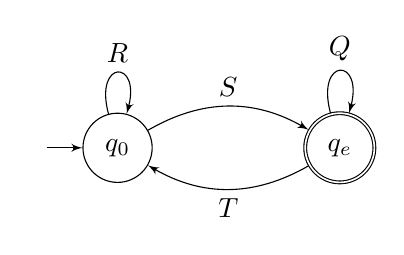
\begin{tikzpicture}[>=latex',/tikz/initial text=""]
	\node (q0) at (0bp,0bp)  [state, initial]   {$q_0$};
	\node (q1) at (80bp,0bp) [state, accepting] {$q_e$};

	\draw [loop above,->] (q0) to node[auto] {$R$} (q0);
	\draw [bend left,->]  (q0) to node[auto] {$S$} (q1);
	\draw [bend left,->]  (q1) to node[auto] {$T$} (q0);
	\draw [loop above,->] (q1) to node[auto] {$Q$} (q1);
\end{tikzpicture}
\\
ki jih prepišemo v en sam regularni izraz oblike:
\[ (R+SQ^*T)^*SQ^* \]

\begin{primeri}
\item Zapiši DKA za preverjanje deljivosti s 3 v binarnem sistemu? Zapiši še regularni izraz.\\
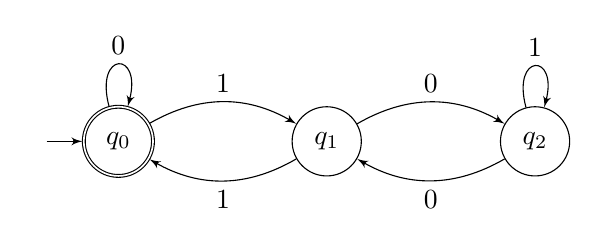
\begin{tikzpicture}[>=latex',/tikz/initial text=""]
	\node (q0) at (0bp,0bp)   [state, initial, accepting] {$q_0$};
	\node (q1) at (75bp,0bp)  [state]                     {$q_1$};
	\node (q2) at (150bp,0bp) [state]                     {$q_2$};

	\draw [loop above,->] (q0) to node[auto] {$0$} (q0);
	\draw [bend left,->]  (q0) to node[auto] {$1$} (q1);
	\draw [bend left,->]  (q1) to node[auto] {$1$} (q0);
	\draw [bend left,->]  (q1) to node[auto] {$0$} (q2);
	\draw [bend left,->]  (q2) to node[auto] {$0$} (q1);
 	\draw [loop above,->] (q2) to node[auto] {$1$} (q2);
\end{tikzpicture}
\ \\
Iz grafa eliminiramo eno stanje in zapišemo regularni izraz:
\[ (0+1(01^*0)^*1)^* \]
Možna pa je še ena rešitev, če eliminiramo drugo stanje.%napiši jo :P
\end{primeri}

\subsect{Desno-linearna gramatika $\rightarrow$ Nedeterministični končni avtomat z $\varepsilon$-prehodi}\label{DLG-eNKA}
Vhodno stanje avtomata je začetni simbol gramatike, nato pa stanja označujemo glede na končne in vmesne simbole, ki jih moramo še porabiti. Produkcije predstavljajo $\varepsilon$ prehode v avtomatu, preostali prehodi avtomata pa so črke, ki jih generiramo.

\Primer{Pretvori podano desno-linearno gramatiko v nedeterministični končni avtomat z $\varepsilon$-prehodi.
\begin{align*}
S &\rightarrow abA\ |\ aS\\
A &\rightarrow aa\ |\ bA\\
\end{align*}
\ \\[-25pt]%lol, hack
Po zgoraj opisanem postopku dobimo:\\ \ \\
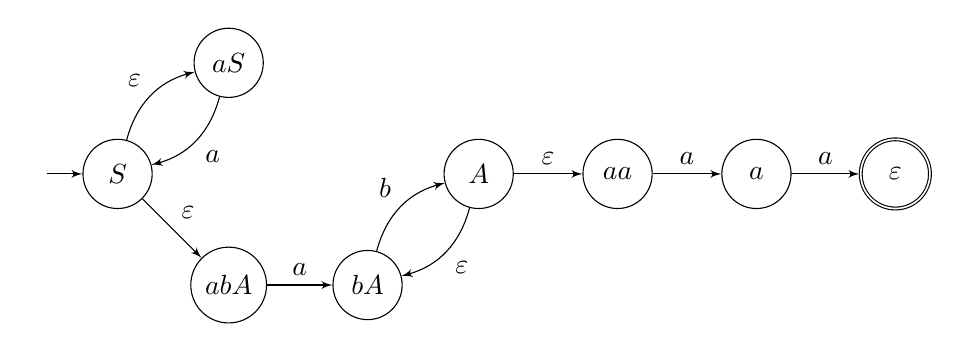
\begin{tikzpicture}[>=latex',/tikz/initial text=""]
	\node (S)   at (0bp,0bp)     [state, initial]  {$S$};
	\node (aS)  at (40bp,40bp)   [state]           {$aS$};
	\node (abA) at (40bp,-40bp)  [state]           {$abA$};
	\node (bA)  at (90bp,-40bp)  [state]           {$bA$};
	\node (A)   at (130bp,0bp)   [state]           {$A$};
	\node (aa)  at (180bp,0bp)   [state]           {$aa$};
	\node (a)   at (230bp,0bp)   [state]           {$a$};
	\node (e)   at (280bp,0bp)   [state,accepting] {$\varepsilon$};

	\draw [bend left,->]  (S) to node[auto] {$\varepsilon$} (aS);
	\draw [bend left,->]  (aS) to node[auto] {$a$} (S);
	\draw [->]  (S) to node[auto] {$\varepsilon$} (abA);
	\draw [->]  (abA) to node[auto] {$a$} (bA);
	\draw [bend left,->]  (bA) to node[auto] {$b$} (A);
	\draw [->]  (A) to node[auto] {$\varepsilon$} (aa);
	\draw [->]  (aa) to node[auto] {$a$} (a);
	\draw [->]  (a) to node[auto] {$a$} (e);
	\draw [bend left,->]  (A) to node[auto] {$\varepsilon$} (bA);
\end{tikzpicture}
}

\sect{Dokazovanje regularnosti jezika}\label{sec:Dokazovanje RJ}
%Dostikrat hočemo sestaviti regularen izraz za določen jezik in niti ne vemo ali je regularen izraz sploh regularen ali ne. Za to imamo nekaj metod za dokazovanje regularnosti jezika.%?false... ne moreš sestavit regularnega izraza, ki ni regularen :)
Kadar ugotavljamo, ali je nek jezik regularen, to lahko naredimo na več načinov:
\begin{items}
\item Pokažemo da je regularen:
	\begin{items}
	\item Jezik skonstruiramo v enem izmed modelov, ki sprejemajo regularne jezike:
		\begin{items}
		\item \nameref{sec:KA}
		\item \nameref{sec:RI}
		\item \nameref{sec:LLGDLG}
		\end{items}
	\end{items}
\item Dokažemo da ni regularen:
	\begin{items}
	\item Z uporabo leme o napihovanju za regularne jezike
	\item Z uporabo izreka Myhill-Nerode
	\item Dokažemo, da jezik ne spada niti v nek širši razred jezikov (glej \ref{sec:Dokazovanje KNJ})
	\end{items}
\end{items}

%?mislim, da je to pokrito tuki pri lemi...
%Opozorilo: Če zapišemo regularni izraz za jezik, ali naredimo končni avtomat, moramo dobro preveriti da ne obstaja kakšen protiprimer. Torej beseda ki je v jeziku in jo končni avtomat ali regularni izraz ne sprejme, ali obratno.\\
%Če nam ne uspe dokaza (da je ali da ni regularni jezik) do konca speljati, to ne moremo vzeti kot dokaz da ravno nasprotno drži. Velja da v takem primeru še nič ne vemo o regularnosti jezika.

\subsect{Lema o napihovanju za regularne jezike}\label{sec:Lema za RJ}
Lemo o napihovanju za regularne jezike uporabljamo za dokazovanje, da nek jezik ne spada v razred regularnih jezikov. 
\Def{Za vsak regularni jezik obstaja neka konstanta $n$, taka, da lahko vsako besedo $w$ iz jezika, daljšo od $n$, razbijemo na tri dele:
	\[ w=u\ v\ z \]
	Pri čemer velja:
	\begin{items}
	\item $|uv| \leq n$
	\item $|v| > 0$
	\item $uv^iz \in L,\ \forall i \geq 0$ (napihovanje)
	\end{items}
}
Ker dokazujemo da jezik ni regularen, moramo torej najti neko besedo, za katero pri napihovanju ne ostanemo znotraj jezika. Če nam tega z izbrano besedo ne uspe dokazati, še nismo dokazali da je jezik regularen -- edini pravi dokaz tega je konstrukcija jezika v enem izmed modelov, ki opisujejo regularne jezike.
\begin{center}
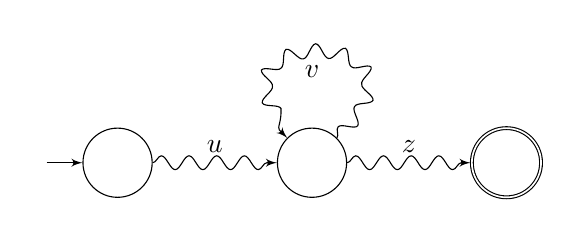
\begin{tikzpicture}[>=latex',/tikz/initial text=""]%scale=0.70, every state/.style={scale=0.70}]
	\node (q0) at (0bp,0bp)  [state, initial]   {};
	\node (q1) at (70bp,0bp) [state]            {};
	\node (q2) at (140bp,0bp) [state, accepting] {};

	\draw [decorate, decoration={snake},->]  (q0) to node[auto] {$u$} (q1);
	\draw [decorate, decoration={snake}, loop,->] (q1) to node[auto] {$v$} (q1);
	\draw [decorate, decoration={snake},->]  (q1) to node[auto] {$z$} (q2);
\end{tikzpicture}
\end{center}
Če zgornjo definicijo pogledamo v kontekstu končnih avtomatov, vidimo, da je $n$ gotovo večji od števila stanj, saj mora za napihovanje v avtomatu obstajati nek cikel, sicer bi bi veljalo $|v|=0$.

\subsect{Izrek Myhill-Nerode}


\subsect{Minimizacija končnih avtomatov}
%\chap{Linearni jeziki}
%nismo delali pri TOR ;)
\sect{Linearne gramatike}\label{sec:LG}
\Def{Linearna gramatika je gramatika, ki ima na desni strani produkcij največ en vmesni simbol.\\
	Definirana kot četvorček $G=\langle N,T,P,S \rangle$, kjer so:
	\begin{items}
	\item N - množica spremenljivk oz. vmesnih simbolov
	\item T - množica znakov oz. končnih simbolov
	\item P - množica produkcij
	\item S - začetni simbol
	\end{items}
}
Posebna primera sta levo in desno-linearne gramatike, ki opisujeta regularne jezike (glej \ref{sec:LLGDLG})%?dvojina: amidoingitrite?
\begin{primeri}
\item Sestavi linearno gramatiko, ki sprejme jezik $L=\{ a^n b^n \ |\ n>0 \}$.
	\[ S \rightarrow aSb\ |\ ab \]
\item Sestavi linearno gramatiko, ki sprejme jezik $L=\{ 1 0^n 1 0^n 1\ |\ n \geq 2 \}$.
	\[ S \rightarrow 100A001 \]
	\[ A \rightarrow 0A0\ |\ 1 \]
\item Sestavi linearno gramatiko, ki sprejme jezik $L=\{ w w^R\ |\ w \in \{ 0,1 \} \}$.
	\[ S \rightarrow 1S1\ |\ 0S0\ |\ \varepsilon \]
\end{primeri}

\chap{Kontekstno-neodvisni jeziki}
\sect{Kontekstno-neodvisne gramatike}
%?oznake, izpeljave, ...
\Def{Kontekstno-neodvisna gramatika je definirana kot četvorček $G=\langle N,T,P,S \rangle$, kjer je:
\begin{items}
\item N - množica spremenljivk oz. vmesnih simbolov
\item T - množica znakov oz. končnih simbolov
\item P - množica produkcij
\item S - začetni simbol
\end{items}
}

%to je še treba nekam umestit
\Def{Kontekstno-neodvisna gramatika je dvoumna, kadar do nekega končnega niza lahko pridemo po več različnih izpeljavah.}

\Def{Kontekstno-neodvisna gramatika je deterministična, kadar za jezik, ki ga gramatika opisuje, obstaja vsaj ena gramatika, ki ni dvoumna. Ni nujno, da je taka gramatika, ki jo imamo - važno je, da taka gramatika obstaja.}

\subsect{Chomskyeva normalna oblika}
\Def{Kontekstno-neodvisna gramatika je v Chomskyevi normalni obliki, kadar nima nekoristnih simbolov, ter so vse produkcije naslednjih dveh oblik:\\
	\[ A \rightarrow a \]
	\[ A \rightarrow BC \]
	\[ a \in T,\ \ B,C \in N \]
}
\subsect{Greibachina normalna oblika}
\Def{Kontekstno-neodvisna gramatika je v Greibachini normalni obliki, kadar so vse produkcije oblike:\\
	\[ A \rightarrow a\gamma\]
	\[ a \in T,\ \ \gamma \in N^* \]
}

\sect{Skladovni avtomati}
\Def{Skladovni avtomat je definiran kot sedmerka $M=\langle Q, \Sigma, \Gamma, \delta, q_0, Z_0, F \rangle$, kjer je:
	\begin{items}
	\item $ Q $ - končna množica stanj
	\item $ \Sigma $ - vhodna abeceda
	\item $ \Gamma $ - skladovna abeceda
	\item $ \delta $ - funkcija prehodov, $\delta : Q \times (\Sigma \cup \{\varepsilon\}) \times \Gamma \rightarrow 2^{Q \times \Gamma^*}$%? zakaj U \varepsilon?
	\item $ q_0 $ - začetno stanje, $q_0 \in Q$
	\item $ Z_0 $ - začetni skladovni simbol, $Z_0 \in \Gamma$
	\item $ F $ - množica končnih stanj
	\end{items}
}
\subsect{Trenutni opis}
\Def{Trenutni opis je trojka $\langle q, w, \gamma \rangle \in Q \times \Sigma^* \times \Gamma^*$, pri čemer je $q$ trenutno stanje, $w$ preostanek vhodnega niza, ter $\gamma$ trenutna vsebina sklada}
\subsect{Relacija $\vdash$}
\Def{Relacija $\vdash$ nas pelje iz enega trenutnega opisa v drugega, če je ta prehod predviden v funkciji prehodov $\delta$:
	\[ \langle q, aw, Z\gamma \rangle \vdash \langle p, w, \gamma'\gamma \rangle \iff \langle p, \gamma' \rangle \in \delta(q,a,Z) \]
}
Uporabljamo tudi posplošeno relacijo $\vdash^*$, ki je ubistvu samo ena ali več-kratna uporaba relacije $\vdash$. Pove nam to, da pridemo iz enega trenutnega opisa do drugega, prek enega ali večih prehodov, pod pogojem, da vse vmesne prehode predvideva funkcija prehodov $\delta$.

\subsect{Jezik skladovnega avtomata}

\sect{Dokazovanje kontekstne-neodvisnosti jezika}\label{sec:Dokazovanje KNJ}
\subsect{Lema o napihovanju za kontekstno-neodvisne jezike}
\subsect{Ogdenova lema za kontekstno-neodvisne jezike}

%\chap{Kontekstno-odvisni jeziki}
\sect{Kontekstno-odvisne gramatike}
\Def{Kontekstno-odvisna gramatika je definirana kot četvorček $G=\langle N,T,P,S \rangle$, kjer so:
	\begin{items}
	\item N - množica spremenljivk oz. vmesnih simbolov
	\item T - množica znakov oz. končnih simbolov
	\item P - množica produkcij
	\item S - začetni simbol
	\end{items}
	Pri tem je:
	\[ P \subset \left[\alpha_1 A \alpha_2 \rightarrow \alpha_1 \gamma \alpha_2 \right],\ 
	 A \in N,\ \ \alpha_1,\alpha_2 \in (N \cup T)^*,\ \ \gamma \in (N \cup T)^+ \]
	Torej, niz z vsaj enim vmesnim simbolom preslikamo v nek drug niz. Pri tem je omejitev, da končnih simbolov ne smemo spreminjati.
}

\begin{primeri}
\item Sestavi kontekstno-odvisno gramatiko, ki sprejme jezik $L=\{ a^n b^n c^n\ |\ n>0 \}$.
	\begin{align*}
	S &\rightarrow aSBC\\
	S &\rightarrow aBC \\
	CB &\rightarrow HB \\
	HB &\rightarrow HC \\
	HC &\rightarrow BC \\
	aB &\rightarrow ab \\
	bB &\rightarrow bb \\
	bC &\rightarrow bc \\
	cC &\rightarrow cc \\
	\end{align*}
	S kompleksnejšo kontekstno-odvisno gramatiko sprejmemo tudi jezik $\{ a^n b^n c^n d^n\ |\ n>0 \}$
\end{primeri}
\subsect{Kurodova normalna oblika}
\Def{Kontekstno-odvisna gramatika je v Kurodovi normalni obliki, kadar so vse produkcije oblike:		\begin{align*}
	AB &\rightarrow CD\\
	A &\rightarrow BC \\
	A &\rightarrow B \\
	A &\rightarrow a \\
	\end{align*}
	\[ a \in T,\ \ A,B,C,D \in N \]
}


%--------------------------------TOR2--------------------------------------

\chap{Turingovi jeziki}
\sect{Zgodovina}
%I've got 23 problems, but a bitch ain't one. -Hilbert, 1900
%\br
Leta 1900 je Nemški matematik David Hilbert objavil seznam triindvajsetih nerešenih problemov v matematiki. Eden izmed Hilbertovih problemov (deseti po vrsti), je vprašanje, ali obstaja postopek, po katerem ugotovimo rešljivost poljubne Diofantske enačbe -- torej, ali lahko ugotovimo, če ima polinom s celoštevilskimi koeficienti $P(x_1, x_2, \dots, x_n)=0$, celoštevilsko rešitev.
%?več zgodovine tu :)
Kljub temu, da je Emil Post že leta 1944 slutil, da je problem nerešljiv, je to dokončno dokazal rus Jurij Matijaševič šele leta 1970 v svojem doktorskem delu. Med reševanjem problema pa so se matematiki že prej začeli ukvarjati s formalizacijo pojma postopka oz. algoritma. Intuitivna definicija tega se glasi nekako tako:
\Def{Algoritem je zaporedje ukazov, s katerimi se v končnem številu korakov opravi neka naloga.}
Pri tem pa ostaja še kar nekaj vprašanj, npr.:
\begin{items}
\item Kakšni naj bodo ukazi? 
	\begin{items}
	\item Osnovni - algoritem ima veliko korakov
	\item Kompleksni - prezapleteni ukazi so že sami algoritmi
	\end{items}
\item Koliko ukazov naj bo?
	\begin{items}
	\item Končno - ali je s končno množico res mogoče rešiti vsako nalogo?
	\item Neskončno - kakšen izvajalec ukazov je sposoben izvršiti neskončno različnih ukazov?
	\end{items}
\item So ukazi zvezni ali diskretni?
\item V kakšnem pomnilniku so ukazi shranjeni?
	\begin{items}%?verjetno ista vprašanja kot pri št. ukazov?
	\item Končnem - ali s končnim zaporedjem ukazov res lahko mogoče rešimo vsako nalogo?
	\item Neskončnem - ali je to praktično uporaben model pomnilnika?
	\end{items}
\end{items}
Nekateri zgodnji poskusi formalizacije pojma algoritma so:%? zgodovinsko zaporedje, letnice, imena modelov, moar info
\begin{items}
    \item Rekurzivne funkcije (Kurt Gödel, Stephen Kleene) 
    \item Splošne rekurzivne funkcije (Jacques Herbrand, Kurt Gödel)
    \item Algoritmi Markova (Andrey Markov, ml.), %sin Markova http://en.wikipedia.org/wiki/Andrey_Markov_(Soviet_mathematician)
    \item Produkcijski sistem (Emil Post), %? je to http://en.wikipedia.org/wiki/Tag_system? 1943?
    \item Lambda račun (Alonso Church, 1936)
    \item Turingov stroj (Alan Turing, 1936)
\end{items}

\pagebreak
\sect{Turingovi stroji}
Turingov stroj se je uveljavil kot uporaben in preprost model računanja, ki zna izračunati vse kar se izračunati da (pod pogojem, da Church-Turingova teza drži). Alan Turing je svoj stroj izpeljal iz razmišljanja o tem, kako človek rešuje miselne probleme na papir. Pri tem je izbral tri sestavne dele:
\begin{items}
\item Nadzorno enoto (glava)
\item Čitalno okno (roka in vid)
\item Trak (papir)
\end{items}
V postopku formalizacije, pa je zaradi večje preprostosti, zahteval še, da je stroj sestavljen iz končno mnogo elementov, ter da deluje v diskretnih korakih.%?končno mnogo elementov? na kaj to cilja?
\ \\
\begin{center}
\begin{tikzturing}
	\node [on chain=trak] {Trak};
	\foreach \x in {1,2,...,5} {
		\node [cell] {$A_{\x}$};
	}
	\node      [cell]           {\ ...\ \ };
	\node (Ai) [cell, selected] {$A_i$};
	\node      [cell]           {\ ...\ \ };
	\node      [cell]           {$A_n$};
	\node      [cell]           {\color{gray}$B$};
	\node      [cell]           {\color{gray}$B$};
	\node      [cell]           {\ ...\ \ };
	\node      [cell, end]      {};

	%?must be a better way, zadnja črta niti ni naravnost
	\node (ne) at (110bp, 70bp) [head, minimum height=1.4cm, minimum width=3cm]  {Nadzorna enota};
	\draw (ne.south) -- (110bp, 25bp) -- (137.5bp, 25bp) [->] to (Ai.north);
	\node [below] at (Ai.south) {Čitalno okno};
\end{tikzturing}
\end{center}

\Def{Turingov stroj je definiran kot sedmerka $M=\langle Q, \Sigma, \Gamma, \delta, q_0, B, F \rangle $, kjer je:
\begin{items}
	\item $Q$ končna množica stanj
	\item $\Sigma$ končna množica vhodnih simbolov, $Q \cap \Sigma = \emptyset$
	\item $\Gamma$ končna množica tračnih simbolov, $\Sigma \subset \Gamma$
	\item $\delta$ funkcija prehodov: $Q \times \Gamma \rightarrow Q \times \Gamma \times \{L,D\}$,\\ kjer $L$ in $D$ označujeta premik levo ali desno
	\item $q_0$ začetno stanje, $q_0 \in Q$
	\item $B$ prazen simbol, $B \in \Gamma$
	\item $F$ množica končnih stanj, $F \subseteq Q$ 
\end{items}}
Stroj deluje tako, da v vsakem koraku opravi naslednje:
\begin{items}
	\item preide v neko stanje
	\item zapiše nov simbol v celico, ki je pod oknom
	\item okno premakne eno celico levo ali desno
\end{items}

\subsect{Trenutni opis}
\Def{$TO = \Gamma^* \times Q \times \Gamma^*$ je množica vseh trenutnih opisov.\\
Nek trenutni opis $\langle \alpha_1, q, \alpha_2 \rangle$, ali krajše $\alpha_1\ q\ \alpha_2$ opisuje konfiguracijo Turingovega stroja.
\br
\begin{center}
\begin{tikzturing}
	\node      [cell, minimum width=3.6cm] {$\alpha_1$};
	\node (Ai) [cell, selected]            {};
	\node      [cell, minimum width=3cm]   {$\alpha_2$\ \ \ };
	\node      [cell]                      {\color{gray}$B$};
	\node      [cell]                      {\color{gray}$B$};
	\node      [cell]                      {\ ...\ \ };
	\node      [cell, end]                 {};

	%?must be a better way, zadnja črta niti ni naravnost
	\node (ne) at (40bp, 60bp) [head]  {$q$};
	\draw (ne.south) -- (40bp, 25bp) -- (60.5bp, 25bp) [->] to (Ai.north);
	%\node [below, minimum width=4cm] at (alpha1.south) {$\alpha_1$};
	%\node [below, minimum width=4cm] at (alpha2.south) {$\alpha_2$\ \ \ \ };
\end{tikzturing}
\end{center}
\br
Čitalno okno je nad prvim znakom niza $\alpha_2$, iz tega lahko razberemo:
\begin{items}
	\item če je $\alpha_1 = \varepsilon$, je okno skrajno levo
	\item če je $\alpha_2 = \varepsilon$, je okno nad $B$ in so naprej sami $B$-ji
\end{items}}

\subsect{Relacija $\vdash$}
\Def{Če sta $u,v$ trenutna opisa iz množice $TO$, ter $v$ neposredno sledi iz $u$ v enem koraku Turingovega stroja, tedaj pišemo $u \vdash v$.
\br
Naj bo $x_1 \dots x_{i-1}\ q\ x_i \dots x_n$ trenutni opis:
\begin{items}
\item če je $\delta(q,x_i) = \langle p,Y,D \rangle$:\\
$x_1 \dots x_{i-1}\ q\ x_i \dots x_n \vdash x_1 \dots x_{i-1}\ Y\ p\ x_{i+1} \dots x_n$
\item če je $\delta(q,x_i) = \langle p,Y,L \rangle$: 
	\begin{items}
	\item če je okno na robu ($i=1$), se Turingov stroj ustavi, ker je trak na levi omejen.
	\item če okno ni na robu ($i>1$), potem: $x_1 \dots x_{i-2} x_{i-1}\ q\ x_i \dots x_n \vdash x_1 \dots\ x_{i-2} p\ x_{i-1}\ Y\ x_{i+1} \dots x_n$
	\end{items}
\end{items}}
Imamo pa tudi posplošeno relacijo $u \vdash^* v$, ki pove, da trenutni opis $v$ sledi iz $u$ v enem ali večih korakih.
\Def{$u \vdash^* v$, če obstaja tako zaporedje $x_i, (i \in [0, 1, \dots, k], k \geq 0)$, da velja $u=x_0, v=x_k$ in $x_0 \vdash x_1 \wedge x_1 \vdash x_2 \wedge \dots \wedge x_{k-1} \vdash x_k$
\br
Torej, trenutni opis $v$ sledi iz $u$, v $k$ korakih Turingovega stroja.}
\sect{Jezik Turingovega stroja}
\Def{Jezik Turingovega stroja je:
\begin{equation*}
L(M) = \{ w\ |\ w \in \Sigma^* \wedge \varepsilon\ q_0\ w \vdash^*\alpha_1\ q_F\ \alpha_2 \wedge \alpha_1,\alpha_2 \in \Gamma^*, q_F \in F \}
\end{equation*}
}
Z besedami to pomeni, da je jezik Turingovega stroja množica besed, ki če jih damo na vhod stroja, povzročijo, da se ta v končno mnogo korakih znajde v končnem stanju.
\ \\
\begin{center}
\begin{tikzturing}
	\node (Ai) [cell, selected]          {};
	\node      [cell, minimum width=4cm] {$w$\ \ \ \ \ };
	\node      [cell]                    {\color{gray}$B$};
	\node      [cell]                    {\color{gray}$B$};
	\node      [cell]                    {\ ...\ \ };
	\node      [cell, end]               {};

	%?must be a better way, zadnja črta niti ni naravnost
	\node (ne) at (90bp, 60bp) [head] {$q_0$};
	\draw (ne.south) -- (90bp, 25bp) -- (0bp, 25bp) [->] to (Ai.north);
\end{tikzturing}
\br
Začetna konfiguracija Turingovega stroja.
\end{center}
\Def{Jezik $L$ je Turingov jezik, če obstaja Turingov stroj $M$, tak, da je $L = L(M)$.}
\subsect{Ugotavljanje pripadnosti besed Turingovemu jeziku}
Pri vprašanju ali je neka beseda v jeziku, Turingove jezike ločimo na:
\begin{items}
\item Odločljive - obstaja algoritem, s katerim se lahko za poljubno besedo odločimo, ali pripada jeziku.
\item Neodločljive - v splošnem ni algoritma, ki bi za poljubno vhodno besedo z DA ali NE odgovoril na vprašanje pripadnosti.
	\begin{items}
	\item če je odgovor DA, to ugotovimo v nekem končnem številu korakov.
	\item če je odgovor NE, pa ni nujno, da se bo stroj kdaj ustavil.
	\end{items}
\end{items}

%?\fixme - vennov diagram beseda w znotraj L kroga... pomojm ne rabmo :P

%?where does this go?
%Terminologija: re (recursively enumerable, Turing recognizable)%?semi-decidable? 
%Rekurzivni jezik (decidable)%?where does this go?

\fixme - vennov diagram odločljivi jeziki znotraj Turingovih?

\Primer{Zapiši Turingov stroj, ki sprejema jezik $L=\{0^n 1^n | n \geq 1\}$\\
	Skica izvajanja stroja:
	\begin{items}
	\item $0^{n}1^{n}$ - vhodna beseda
	\item $X0^{n-1}1^{n}$ - zamenjamo najbolj levo $0$ z $X$
	\item $X0^{n-1}Y1^{n-1}$ - premaknemo okno desno do najbolj leve $1$ in jo zamenjamo z $Y$
	\item $XX0^{n-2}Y1^{n-1}$\\ 
		$XX0^{n-2}YY1^{n-2}$ - ponovimo in vidimo, da bomo niz sprejeli, če je prave oblike.
	\end{items}
	Turingov stroj zapišemo kot $M=\langle Q,\Sigma,\Gamma,\delta,q_0,B,F \rangle$:
	\begin{items}
    \item $Q=\{ q_0,q_1,q_2,q_3,q_4 \}$
    \item $\Sigma = \{ 0,1 \}$
    \item $\Gamma = \{ 0,1,B,X,Y \}$
    \item $F = \{ q_4 \}$
    \item $\delta$ bomo definirali s tabelo
	\end{items}

    Pomen stanj:
    \begin{items}
    \item $q_0$ - začetno stanje in stanje pred zamenjavo 0 z X
    \item $q_1$ - premikanje desno do 1
    \item $q_2$ - zamenjava 1 z Y in premikanje levo do X
    \item $q_3$ - najde X in se premik desno
    \item $q_4$ - končno stanje
    \end{items}

    Tabela prehajanja stanj:\\
	\begin{center}
    \begin{tabular}{ c | c c c c c}
	& 0 & 1 & X & Y & B\\ \hline
	$q_0$& $\langle q_1,X,D\rangle$ & -- & -- & $\langle q_3,Y,D\rangle$ & --\\
	$q_1$& $\langle q_1,0,D\rangle$ & $\langle q_2,Y,L\rangle$ & -- & $\langle q_1,Y,D\rangle$ & --\\
	$q_2$& $\langle q_2,0,D\rangle$ & -- & $\langle q_0,X,D\rangle$ & $\langle q_2,Y,L\rangle$ & --\\
	$q_3$& -- & -- & -- & $\langle q_3,Y,D\rangle$ & $\langle q_4,B,D\rangle$\\
	$q_4$& -- & -- & -- & -- & --\\
	\end{tabular}
	\end{center}
	\br
	Izvajanje stroja s trenutnimi opisi:
	\[ q_0 0011 \vdash X q_1 011 \vdash X 0 q_1 11 \vdash X q_2 0 Y 1 \vdash \dots \]
}
%?zapiski 2007 imajo tu še nekaj o turingovih jezikih
\subsect{Turingov stroj kot računalnik funkcij}
Imamo Turingov stroj, ki ima na traku neko število ničel, ki predstavljajo pozitivna naravna števila, ločena z enicami:
%	\[ 0^{i_1} 1 0^{i_2} 1  \dots 1 0^{i_k} \]
%?skupine ničel so i_1, i_2, ..., kjer so i naravna števila (mjbi i+1 ničel)  
\ \\
\begin{center}
\begin{tikzturing}
	\node (Ai) [cell, selected]            {};
	\node      [cell, minimum width=2cm]   {$0^{i_1}$\ \ \ };
	\node      [cell]                      {$1$};
	\node      [cell, minimum width=1.4cm] {$0^{i_2}$};
	\node      [cell]                      {$1$};
	\node      [cell]                      {\ ...\ \ };
	\node      [cell]                      {$1$};
	\node      [cell, minimum width=2.6cm] {$0^{i_k}$\ \ \ \ };
	\node      [cell]                      {\color{gray}$B$};
	\node      [cell]                      {\color{gray}$B$};
	\node      [cell]                      {\ ...\ \ };
	\node      [cell, end]                 {};

	%?must be a better way, zadnja črta niti ni naravnost
	\node (ne) at (70bp, 60bp) [draw, minimum width=2cm, minimum height=1.2cm]  {$q_0$};
	\draw (ne.south) -- (70bp, 25bp) -- (0bp, 25bp) [->] to (Ai.north);
\end{tikzturing}
\end{center}
Recimo, da se stroj po nekem številu korakov ustavi in ima na traku skupino ničel $0^m$, na levi in desni strani skupine pa same $B$-je. S tem je stroj morda izračunal neko funkcijo:
	\[ f^{(k)}:\mathbb{N}_+^k \rightarrow \mathbb{N}_+ \mbox{\ \ oz. \ \ } f(i_1, i_2, \dots, i_k) = m \]
%?\fixme - slika TS s skupino ničel na traku\br... pomojm ne rabmo :P
Funkcija $f$ ni nujno definirana za vsako $k$-terico iz $\mathbb{N}_+^k$, torej je parcialna funkcija, kadar pa je definirana povsod, pravimo da je totalna. Stroj se pri nedefiniranih $k$-tericah pač na neki točki ustavi in pri tem na traku ne pusti le ene skupine ničel, ali pa se sploh ne ustavi.
Isti turingov stroj hkrati računa več funkcij: $f^{(1)}, f^{(2)}, \dots f^{(k)}$.%?računa ali "lahko računa".. ne štekam ubistvu čist

\subsubsection{Parcialna rekurzivna funkcija}
\Def{Vsaka funkcija $f^{(k)}:\mathbb{N}_+^k \rightarrow \mathbb{N}$, ki jo lahko izračuna nek Turingov stroj, je parcialna rekurzivna funkcija. Če je $f^{(k)}$ definirana za vse $k$-terice, jo imenujemo totalna rekurzivna funkcija (včasih samo rekurzivna funkcija)}
Vse običajne aritmetične funkcije so parcialne ali celo totalne rekurzivne funkcije. V primerih si bomo pogledali nekaj primerov, tu pa jih nekaj naštejmo: $m+n,\ m*n,\ n!,\ 2^n,\ \lceil \log(n) \rceil,\ m^n,\ \dots$.
%so najdl primer, ki ne spada sem z diagonalizacijo
%na začetku so gledali totalne... pa so vidl da morajo parcialne
\begin{primeri}
\item
    Ali je $f(m,n)=m+n$ (parcialno) rekurzivna?\\
    Skica stroja, ki računa $m+n$:
    \begin{items}
    \item $0^m 1 0^m$ - vhodna beseda
    \item $B0^{m-1} 1 0^m$ - izbriši prvo ničlo
    \item $B0^{m+n}$ - premakni se do 1 in jo zamenjaj z 0
    \end{items}%?DN naredi cel stroj
\item
    Ali je $f(m,n)=m*n$ (parcialno) rekurzivna?\\
    Skica stroja, ki računa $m*n$:
    \begin{items}
    \item $0^m 1 0^n$ - vhodna beseda
    \item $0^m 1 0^n 1$ - premakni se na konec in zapiši 1 (ločnica za rezultat)
    \item $B 0^{m-1} 1 0^n 1$ - premakni se na začetek in izbriši 0
    \item $B 0^{m-1} 1 0^m 1 0^n$ - prekopiraj $n$ ničel za ločnico (in ničle)
    \item $B^{m} 1 0^m 1 0^{m*n}$ - ponavljaj tadva koraka, dokler ni več ničel pred prvo 1
    \item $B^{m+n+2}0^{m*n}$ - izbriši del, ki ne spada v rezultat 
    \end{items}%?naredi cel stroj
\end{primeri}

\sect{Razširitve Turingovega stroja}
V tem odseku bomo spoznali nekaj razširitev Turingovega stroja in pokazali da so enako močne kot osnovni model. Poleg tega bomo naredili še pregled alternativnih modelov, za katere se je tudi izkazalo, da so enako močni.%, nato pa si bomo ogledali še nekaj stvari, ki jih Turingov stroj kljub vsemu ne more izračunati.

\Odmakni{Postopek dokazovanja}{Recimo, da je $\mathcal{M}$ razred modelov, za katerega želimo dokazati, da je ekvivalenten razredu Turingovih strojev. Poiskati moramo sistematičen, končen postopek S, ki poljubnemu stroju $M \in \mathcal{M}$ priredi nek Turingov stroj $M'$, ki je sposoben simulirati $M$.
\begin{center}
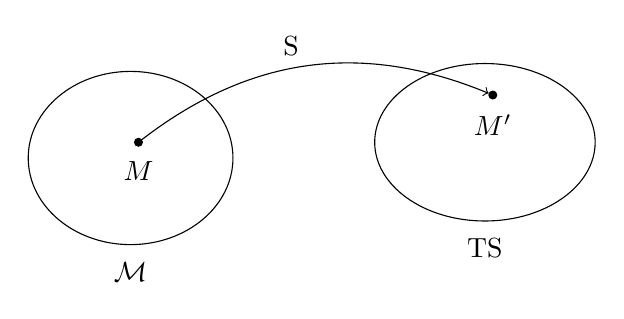
\begin{tikzpicture}[vert/.style={circle, draw,fill=black, inner sep=1pt}]
	\node (l) [vert] at (0.1cm, 0.2cm) {};
	\node [below=2pt] at (l.south) {$M$};
	\node (r) [vert] at (4.6cm, 0.8cm) {};
	\node [below=2pt] at (r.south){$M'$};

	\draw (0cm,0cm) ellipse (1.3cm and 1.1cm) node(le) {};
	\node at (le) [below=1.2cm] {$\mathcal{M}$};
	\draw (4.5cm,0.2cm) ellipse (1.4cm and 1.0cm) node(re) {};
	\node at (re) [below=1.1cm] {TS};

	\draw [bend left, ->] (l) to node[auto] {S} (r);
\end{tikzpicture}
\end{center}}
\subsect{Nadzorna enota kot pomnilnik}
Vsako stanje stroja je sestavljeno iz dveh delov -- stanja avtomata in shrambe za tračne znake. Novo množico stanj zapišemo kot $Q=K\times\Gamma$, kjer je $K$ stara množica stanj in $\Gamma$ tračna abeceda.
\Primer{Sestavi Turingov stroj za razpoznavanje besed, pri katerih se prvi znak ne ponovi:\\
	Stroj $M=\langle Q,\Sigma,\Gamma,\delta,q_0,B,F \rangle$ zapišemo kot:
	\begin{items}
	\item $M=\langle Q, \{0,1\}, \{0,1,B\}, \delta, \langle q_0, B \rangle, B, F \rangle$
	\item $Q=\{ q_0, q_1 \} \times \{0,1,B\} = \{ \langle q_0, 0\rangle , \langle q_0, 1\rangle , \langle q_0, B\rangle , \langle q_1, 0\rangle , \langle q_1, 1\rangle , \langle q_1, B\rangle\} $
	\item $F=\{ \langle q_1, B \rangle \}$
	\item $\delta$ zapišemo kot:
		\begin{items}
		\item Shrani prvi znak besede v stanje stroja:\\
			$\delta(\langle q_0, B\rangle, 0) = \langle\langle q_1, 0 \rangle, 0, D\rangle$\\
			$\delta(\langle q_0, B\rangle, 1) = \langle\langle q_1, 1 \rangle, 1, D\rangle$
		\item Premakni okno v desno do prvega znaka, enakega shranjenemu:\\
			$\delta(\langle q_1, 0\rangle, 1) = \langle\langle q_1, 0 \rangle, 1, D\rangle$\\
			$\delta(\langle q_1, 1\rangle, 0) = \langle\langle q_1, 1 \rangle, 0, D\rangle$
		\item Če prebereš $B$, pojdi v končno stanje:\\
			$\delta(\langle q_1, 0\rangle, B) = \langle\langle q_1, B \rangle, karkoli \rangle$\\
			$\delta(\langle q_1, 1\rangle, B) = \langle\langle q_1, B \rangle, karkoli \rangle$
		\item Sicer se ustavi. To dosežemo tako, da ne definiramo prehodov:\\
			$\delta(\langle q_1, 0\rangle, 0)$ in $\delta(\langle q_1, 1\rangle, 1)$
		\end{items}
	\end{items}
}
\subsect{Večsledni trak}
Na traku imamo več kot eno sled, kar pomeni, da s traku beremo $k$-terice tračnih znakov, kar zapišemo kot: $\Gamma=\Gamma_1\times\Gamma_2\times\dots\times\Gamma_k$.
\ \\
\begin{center}
\begin{tikzturing}
	\node (Ai) [cell1, selected] {$A1_{0}$};
	\node at (0bp,-0.6cm) [cell2, selected] {$A2_{0}$};
	\node at (0bp,-1.2cm) [cell3, selected] {$A3_{0}$};

	\foreach \x in {1,2,3} {
		\node [cell1] {$A1_{\x}$};
		\node [cell2] {$A2_{\x}$};
		\node [cell3] {$A3_{\x}$};
	}

	\node [cell1] {\ ...\ \ };
	\node [cell2]  {\ ...\ \ };
	\node [cell3]  {\ ...\ \ };

	\node [cell1, end] {};
	\node [cell2, end] {};
	\node [cell3, end] {};

	%?must be a better way, zadnja črta niti ni naravnost
	\node (ne) at (40bp, 60bp) [draw, minimum width=2cm, minimum height=1.2cm]  {$q_0$};
	\draw (ne.south) -- (40bp, 25bp) -- (0bp, 25bp) [->] to (Ai.north);
\end{tikzturing}
\end{center}

\Primer{Sestavi Turingov stroj, ki preveri, ali je vhodno število praštevilo.\\
	Skica stroja:
	\begin{items}
	\item Trak ima tri sledi:
		\begin{items}
		\item na prvi sledi je vhodno število
		\item na drugi sledi je števec, ki na začetku hrani število 2
		\item tretjo sled uporabimo za delovno sled, na začetku je lahko prazna.
		\end{items}
	\item Stroj deluje tako:
		\begin{items}
		\item prepiši število s prve sledi na tretjo sled
		\item odštevaj število iz druge sledi od števila na tretji sledi
		\item če se odštevanje konča z 0, se ustavi (ni praštevilo)
		\item sicer število na drugi sledi povečaj za 1
		\item če je število na drugi sledi enako tistemu na prvi, sprejmemo (je praštevilo)
		\item sicer, ponovimo postopek
		\end{items}
	\end{items}
}
\subsect{Prestavljanje vsebine traku}
Recimo, da bi s traku radi vzeli nekaj zaporednih znakov tako, kot da bi jih izrezali iz traku in nato trak zlepili nazaj skupaj, izrezane simbole pa bi si pri tem seveda radi nekako zapomnili. Tudi to metodo realiziramo s pomočjo shrambe za tračne simbole v nadzorni enoti, a moramo pri tem paziti, da je funkcija prehodov pravilno napisana.
\br\fixme slika "gube" na traku in slika nadzorne enote
\Primer{Sestavi Turingov stroj, ki premakne vsebino traku za 2 celici v desno.\\
	Skica stroja:
	\begin{items}
    \item $Q$ vsebuje stanja oblike: $\langle q, A_1, A_2 \rangle;\ q \in \{ q_1, q_2 \},\ A_1, A_2 \in \Gamma$
    \item $\Gamma$ poleg ostalih znakov, vsebuje še poseben znak $X$, ki označuje izpraznjeno celico na traku
	\item $F=\{ q_2 \}$
	\item $\delta$ zapišemo kot:
		\begin{items}
		\item Prva koraka -- zapomni si in izprazni prvi in drugi znak:\\
			$\delta(\langle q_1, B, B\rangle, A_1) = \langle\langle q_1, B, A_1 \rangle, X, D \rangle $\\
			$\delta(\langle q_1, B, A_1\rangle, A_2) = \langle\langle q_1, A_1, A_2 \rangle, X, D \rangle $
		\item Zapomni si nov znak in prvega iz shrambe zapiši na trak:\\
			$\delta(\langle q_1, A_i, A_{i+1}\rangle, A_{i+2}) = \langle\langle q_1, A_{i+1}, A_{i+2} \rangle, A_i, D \rangle $
		\item Zadnja koraka -- zapiši vsebino shrambe na trak:\\
			$\delta(\langle q_1, A_{n-1}, A_{n}\rangle, B) = \langle\langle q_1, A_{n}, B \rangle, A_{n-1}, D \rangle $\\
			$\delta(\langle q_1, A_{n}, B\rangle, B) = \langle\langle q_2, B, B \rangle, A_{n}, L \rangle $
		\end{items}
	\end{items}
}

%?\fixme ... tu je razlagal tisto neizračunljivo funkcijo nad matrikami. btw, @zidar: poglej tor2-dodatno.pdf - tam govori o preroku

\subsect{Podprogrami}
\fixme
%?Imamo neka posebna stanja, ki signalizirajo vhod in izhod iz podprograma%?je tu govoril o dveh strojih?

\subsect{Turingov stroj z dvosmernim trakom}
Imamo Turingov stroj, ki ima trak neomejen v obe smeri. Vhodna beseda je na začetku napisana nekje na traku, okno pa je na prvem znaku besede.

%kako zbrišem črto pri prvem ...?
\begin{center}
\begin{tikzturing}
	\node      [cell]                    {\ ...\ \ };
	\node      [cell]                    {\color{gray}$B$};
	\node      [cell]                    {\color{gray}$B$};
	\node (Ai) [cell, selected]          {};
	\node      [cell, minimum width=4cm] {$w$\ \ \ \ \ };
	\node      [cell]                    {\color{gray}$B$};
	\node      [cell]                    {\color{gray}$B$};
	\node      [cell]                    {\ ...\ \ };
	\node      [cell, end]               {};

	%?must be a better way, zadnja črta niti ni naravnost
	\node (ne) at (95bp, 60bp) [draw, minimum width=2cm, minimum height=1.2cm]  {$q_0$};
	\draw (ne.south) -- (95bp, 25bp) -- (53.5bp, 25bp) [->] to (Ai.north);
\end{tikzturing}
\end{center}
\ \\
Stroj je definiran skoraj enako kot osnovni Turingov stroj, le funkcija prehodov $\delta$ je enostavnejša, saj ni treba skrbeti, kaj se zgodi, če zadanemo levi rob, kot pri običajnem Turingovemu stroju.
\br
\Trditev{Turingov stroj z dvosmernim trakom ni šibkejši od osnovnega Turingovega stroja.}
\Dokaz{Stroj se lahko vede kot da je omejen na levi. Na začetku izvajanja se premaknemo levo, zapišemo poseben znak, ki nam pomeni konec traku. Nato se premaknemo desno in stroj normalno izvajamo.}%to smo delali tudi na vajah - check it
\ \\
\Trditev{Turingov stroj z dvosmernim trakom ni močnejši od osnovnega.}
\Dokaz{Imamo Turingov stroj $M$ z dvosmernim trakom:
\ \\
%kako zbrišem črto pri prvem ...?
\begin{center}
\begin{tikzturing}
	\node [cell] {\ ...\ \ };

	\foreach \x in {-3,-2,-1} { \node [cell] {$A_{\x}$}; }
	\node (Ai) [cell, selected] {$A_{0}$};
	\foreach \x in {1,2,3} { \node [cell] {$A_{\x}$}; }

	\node [cell] {\ ...\ \ };
	\node [cell, end]      {};

	%?must be a better way, zadnja črta niti ni naravnost
	\node (ne) at (70bp, 60bp) [draw, minimum width=2cm, minimum height=1.2cm]  {$q_0$};
	\draw (ne.south) -- (70bp, 25bp) -- (95bp, 25bp) [->] to (Ai.north);
\end{tikzturing}
\end{center}
\ \\
Stroju $M$ priredimo dvosledni Turingov stroj $M'$. Zgornja sled nam bo predstavljala celice od $A_0$ naprej, spodnja pa vse tiste, levo od $A_0$:
\ \\
\begin{center}
\begin{tikzturing}
	\node (Ai) [cell1, selected] {$A_{0}$};
	\node at (0bp,-0.6cm) [cell2, selected] {\#};

	\foreach \x in {1,2,3} {
		\node [cell1] {$A_{\x}$};
		\node [cell2] {$A_{-\x}$};
	}

	\node [cell1] {\ ...\ \ };
	\node [cell2]  {\ ...\ \ };

	\node [cell1, end] {};
	\node [cell2, end] {};

	%?must be a better way, zadnja črta niti ni naravnost
	\node (ne) at (40bp, 60bp) [draw, minimum width=2cm, minimum height=1.2cm]  {$q_0$};
	\draw (ne.south) -- (40bp, 25bp) -- (0bp, 25bp) [->] to (Ai.north);
\end{tikzturing}
\end{center}

Stroj $M'$ deluje tako:
\begin{items}
\item naeenkrat dela le z eno sledjo
\item ko na drugi sledi vidi \#, zamenja aktivno sled
\item na zgornji sledi dela enako kot $M$
\item na spodnji se obrne smer premikanja
\end{items}
%(tu smo pomojem napisali še 2x isto)

%Formalizacija... ne bomo delal

%Sklep.. sta ekvivalentna - kar izračuna dvosmerni, lahko tudi osnovni.
%Izrek: Za jezik L obstaja TS z dvosmernim trakom, n.t.k., za L obstaja osnovni TS.

%nekdo je vprašal, če je bijekcija, pa je rekel, da ne čist?
}

\subsect{Večtračni Turingov stroj}
Večtračni Turingov stroj ima $k>1$ trakov, ki so neomejeni v obe smeri. Vsak trak ima svoje okno, ki se lahko na vsakem koraku premakne neodvisno od ostalih. Na prvem traku imamo na začetku ponovno vhodno besedo, okno prvega traku pa na prvem znaku vhodne besede. Ostali trakovi so prazni.

\begin{center}
\begin{tikzturing}[cell11/.style={cell1,fill=white}, cell22/.style={cell2,fill=white}]
	\node [cell11] {\ ...\ \ };
	\node at (0bp,-1.5cm) [cell22]  {\ ...\ \ };
	\node at (0bp,-3.0cm) [cell3]  {\ ...\ \ };

	\node (Ai) [cell11, selected] {$w_{0}$};
	\node (Ai2) [cell22, selected] {\color{gray}$B$};
	\node (Ai3) [cell3, selected] {\color{gray}$B$};

	%?must be a better way, zadnja črta niti ni naravnost
	\node (ne) at (67bp, 60bp) [draw, minimum width=2cm, minimum height=1.2cm]  {$q_0$};
	\draw (ne.south) -- (67bp, 25bp) -- (29bp, 25bp) [->] to (Ai.north);
	\draw (ne.south) -- (67bp, -20bp) -- (29bp, -20bp) [->] to (Ai2.north);
	\draw (ne.south) -- (67bp, -65bp) -- (29bp, -65bp) [->] to (Ai3.north);

	\foreach \x in {1,2,3} {
		\node [cell11] {$w_{\x}$};
		\node [cell22] {\color{gray}$B$};
		\node [cell3] {\color{gray}$B$};
	}

	\node [cell11] {\ ...\ \ };
	\node [cell22]  {\ ...\ \ };
	\node [cell3]  {\ ...\ \ };

	\node [cell11, end] {};
	\node [cell22, end] {};
	\node [cell3, end] {};
\end{tikzturing}
\end{center}

\Def{Korak stroja $\delta$ opišemo kot:
	\[\delta = Q \times \Gamma^k \rightarrow Q\times(\Gamma\times\{ L,D,- \})^k \]
        Na vsakem koraku torej iz trenutnega stanja in tračnega simbola na vsakem traku dobimo neko novo stanje ter za vsak trak neodvisno nov simbol in premik.}

\Trditev{Večtračni Turingov stroj je enako močen kot osnovni model.}
\Dokaz{
	\Odmakni{($\Rightarrow$)}{Večtračni Turingov stroj uporabi le prvi trak.}
	\Odmakni{($\Leftarrow$)}{Turingovemu stroju $M$ s $k$-trakovi priredimo $2k$-sledni v obe strani neskončni Turingov stroj $M'$.
	Za vsak trak stroja $M$ imamo tako dve sledi v $M'$ -- na zgornji sledi je zapisana oznaka $X$, ki pove, kje naj bi bilo okno na tem traku stroja $M$, na spodnji sledi pa je zapisana vsebina tega traku stroja $M$.

\begin{center}
\begin{minipage}[t]{6cm}
\begin{tikzturing}[cell11/.style={cell1,fill=white}]
	\node [cell11] {\ ...\ \ };
	\node at (0bp,-1.5cm) [cell2]  {\ ...\ \ };

	\node (Ai) [cell11, selected] {$a$};

	\node       [cell2] {$c$};
	\node (Ai2) [cell2, selected] {$d$};

	%?must be a better way, zadnja črta niti ni naravnost
	\node (ne) at (50bp, 60bp) [draw, minimum width=2cm, minimum height=1.2cm]  {$q$};
	\draw (ne.south) -- (50bp, 25bp) -- (29bp, 25bp) [->] to (Ai.north);
	\draw (ne.south) -- (50bp, 25bp) -- (57bp, 25bp) [->] to (Ai2.north);

	\node [cell11] {$b$};

	\node [cell11] {\color{gray}$B$};
	\node [cell2]  {\color{gray}$B$};

	\node [cell11] {\ ...\ \ };
	\node [cell2]  {\ ...\ \ };

	\node [cell11, end] {};
	\node [cell2, end] {};
\end{tikzturing}
$k$-tračni stroj $M$
\end{minipage}
\begin{minipage}[t]{6cm}
\begin{tikzturing}
	\node [cell1] {\ ...\ \ };
	\node at (0bp,-0.6cm) [cell2]  {\ ...\ \ };
	\node at (0bp,-1.2cm) [cell3]  {\ ...\ \ };
	\node at (0bp,-1.8cm) [cell4]  {\ ...\ \ };

	\node [cell1] {$X$}; \node [cell1] {\color{gray}$B$};
	\node [cell2] {$a$}; \node [cell2] {$b$};
	\node [cell3] {\color{gray}$B$}; \node [cell3] {$X$};
	\node [cell4] {$c$}; \node [cell4] {$d$};

	\node (Ai) [cell1,selected] {\color{gray}$B$};
	\node      [cell2,selected] {\color{gray}$B$};
	\node      [cell3,selected] {\color{gray}$B$};
	\node      [cell4,selected] {\color{gray}$B$};

	\node [cell1] {\ ...\ \ };
	\node [cell2] {\ ...\ \ };
	\node [cell3] {\ ...\ \ };
	\node [cell4] {\ ...\ \ };

	\node [cell1, end] {};
	\node [cell2, end] {};
	\node [cell3, end] {};
	\node [cell4, end] {};

	%?must be a better way, zadnja črta niti ni naravnost
	\node (ne) at (60bp, 60bp) [draw, minimum width=2cm, minimum height=1.2cm]  {$q$};
	\draw (ne.south) -- (60bp, 25bp) -- (85.5bp, 25bp) [->] to (Ai.north);

\end{tikzturing}
$2k$-sledni stroj $M'$
\end{minipage}
\end{center}
\br

Stroj $M'$ torej hrani trenutni položaj na trakovih z dodatno sledjo, ki ima v ustrezni celici zapisan simbol $X$.
\br
Poleg tega pa pri $M'$ potrebujemo še drugačno nadzorno enoto, ki hrani:
\begin{items}
\item Stanje stroja
\item $k$ tračnih simbolov
\item Števec na intervalu $[0,k]$, ki nam pove, koliko simbolov $X$ je še desno od trenutnega položaja okna.
\end{items}
\ \\
Stroj $M'$ simulira en korak stroja $M$ tako da:
\begin{items}
\item Okno pomika v desno
\item Ko na neki sledi naleti na simbol $X$:
	\begin{items}
	\item V nadzorno enoto shrani simbol iz naslednje sledi
	\item Zmanjša števec za 1.
	\end{items}
\item Ko števec doseže 0, se začne pomikati v levo
\item Ko naleti na simbol $X$
	\begin{items}
	\item Zamenja tračni simbol na naslednji sledi, enako kot bi naredil stroj $M$
	\item Premakne se levo ali desno, enako kot bi naredil stroj $M$
	\item Poveča števec za 1
	\end{items}
\item Ko števec doseže $k$, nadzorna enota preide v novo stanje, enako kot bi stroj $M$
\end{items}
\ \\
En korak stroja $M$ torej simuliramo s končno dolgim sprehodom v desno in levo.
}}%konec dokaza


\subsect{Nedeterministični Turingov stroj}
Pri nedeterminističnemu Turingovemu stroju, imamo lahko v določeni konfiguraciji več možnosti, kako bo stroj nadaljeval z delom. Za formalni zapis tega je potrebno spremeniti le funkcijo prehodov $\delta$, ki sedaj slika v množico konfiguracij, namesto v eno samo:\\
 \[ \delta:Q\times\Gamma \rightarrow 2^{Q\times\Gamma\times\{ L,D,- \}} \]

\Def{Nedeterministični Turingov stroj sprejme besedo natanko tedaj, kadar obstaja končno zaporedje korakov, po katerem pridemo do končnega stanja.}

\Primer{%nekoliko lame primer... where's the action :)
$\delta(0, a) = \{ \langle q_1, b, L \rangle, \langle q_2, c, D \rangle, \langle q_3, a, L \rangle, \langle q_2, B, L \rangle \}$\\
Stroj bo izbral tisto preslikavo, ki ga vodi k sprejetju vhodne besede. Če to ni mogoče, se bo stroj ali ustavil v nekončnem stanju, ali pa se sploh ne bo ustavil.
}

\Trditev{Nedeterministični Turingov stroj zmore vse kar zmore osnovni Turingov stroj.}
\Dokaz{Funkcija prehodov $\delta$ osnovnega TS je le poseben primer funkcije $\delta$ nedeterminističnega Turingovega stroja.}
\Trditev{Nedeterministični Turingov stroj ni močnejši od osnovnega modela.}

\Dokaz{Simulacija nedeterminističnega Turingovega stroja z osnovnim:\\
%slika 
%
% d     a
%   |-------
% q |   o
%
%
\fixme slika\\
Naj bo $M$ nek nedeterministični Turingov stroj in naj ima njegov program v vsaki mmnožici $\delta(q,a)$ največ $r$ možnih potez, kjer je $r$ končno število.\\
Stroju $M$ priredimo osnovni 3-sledni Turingov stroj $M'$, z naslednjimi lastnostmi:
\begin{items}
\item na prvi sledi ima abecedo stroja $M$
\item na drugi sledi generira zaporedje navodil besed nad abecedo $\{1, 2, \dots, r\}$ v leksikografskem vrstnem redu (npr. $r = 3: 1,2,3,11,12,13,\dots)$
\item na tretji sledi simulira stroj $M$, kot da bi ta izbral poteze skladno s tekočimi navodili
\end{items}
Natančneje stroj $M'$ deluje tako:
\begin{items}
\item na drugi sledi sestavi novo, naslednje navodilo
\item prepiše vhodno besedo s prve na tretjo sled
\item na tretji sledi simulira stroj $M$, kot da bi ta izbral svoje poteze skladno s tekočimi navodili.\\
      Pri tem:
      \begin{items}
      \item če $M'$ pride do konca navodila in je tedaj v končnem stanju, vhodno besedo sprejme in konča, kot bi to storil tudi $M$
      \item sicer nadaljuje s prvim korakom ali pa se ustavi v končnem stanju
      \end{items}
\end{items}
}
\Trditev{Če $M$ sprejme besedo jo sprejme tudi $M'$.}
\Izrek{Za jezik $L$ obstaja nedeterministični Turingov stroj natanko tedaj, ko za $L$ obstaja osnovni Turingov stroj.}

\subsect{Večdimenzionalni Turingov stroj}
Pri tem modelu je trak k-dimenzionalen ($k \geq 2$) in je v vsaki dimenziji neomejen v obe smeri.\\
Za tridimenzionalni Turingov stroj bi to pomenilo, da je celica kocka in se po vsakem koraku stroja premaknemo v eno izmed šestih sosednjih celic.

\subsect{Turingov stroj z več okni}
Nadzorna enota hkrati lahko bere iz večih oken na istem traku.\\
Okna so ves čas enako oddaljena med seboj.
\br
\begin{tikzturing}
	\node [cell1, minimum width=2cm] {};

	\node (Ai) [cell1,selected] {$A_i$};
	\node [cell1, minimum width=1.7cm] {\ ...\ \ };
	\node (Ai2) [cell1,selected] {$A_j$};
	\node [cell1, minimum width=1cm] {\ ...\ \ };
	\node (Ai3) [cell1,selected] {$A_k$};
	\node [cell1, minimum width=2cm] {};

	%?must be a better way, zadnja črta niti ni naravnost
	\node (ne) at (80bp, 60bp) [draw, minimum width=2cm, minimum height=1.2cm]  {$q$};
	\draw (ne.south) -- (80bp, 30bp) [->] to (Ai.north);
	\draw (ne.south) -- (80bp, 30bp) [->] to (Ai2.north);
	\draw (ne.south) -- (80bp, 30bp) [->] to (Ai3.north);
\end{tikzturing}

%-----------------------predavanja 4-------------------------------
%Turing se je zgledoval po človeku

%drugi po funkcijah
%kaj je računanje, izračunljivost, algoritem... na številsko-teoretskih funkcijah f:N->N ... totalne/parcialne
%študirali so totalne f:N->N
%Cilji: storga mat. definicija pojmov s tem da zadosti 2 stvarem:
	%zajeti mora vse "izračunljve funkcije" (vse kar si lahko zamislimo kot problem za računanje)
	%za vsako tako f, mora biti razviden mehaničen postopek za izračun njenih vrednosti
%(HK,HG,lambda)

%zgledovanje po (naravnem) jeziku
%Postov stroj, Algoritmi Markova
%računanje oz. reševanje mat. problemov je pri človeku preoblikovanje množice besed v drugo (opis problema, v opis rešitve)
\sect{Alternative Turingovemu stroju}
Alternative smo našteli že na začetku poglavja. Tu v uvodu na hitro povejmo malo o tem, prek katerih metafor so različni raziskovalci prišli do svojih modelov. Turing je poskušal formalizirati kako človek rešuje problem na papir, ostali pa so se zgledovali po jeziku (npr. kako iz opisa problema dobiti opis rešitve), ali pa kar po funkcijah.

\subsect{Rekurzivne funkcije (Gödel, Kleene)}
Gödel si je zamislil, da bi iz nekaj osnovnih funkcij z nekaj pravili lahko izpeljal kompleksnejše funkcije. Definiral je: ničelno funkcijo, funkcijo naslednik in projekcijo, ter pravili za sestavljanje: kompozicijo in primitivno rekurzijo.
\br
\fixme začetne in drevo ven%grafek vseh sestavljivih (primitivno rekurzivnih) funkcij \_/
\br
Konstrukcija funkcije opisuje tudi mehanični postopek za izračun vrednosti funkcije tako, da je s tem tudi kandidat za formalni opis pojma algoritma.
\br
Kasneje se je izkazalo, da ta pravila ne zadostujejo, saj obstaja npr. Ackermannova funkcija, ki narašča hitreje od vsake funkcije, ki pripada primitivno rekuzivnim:
\[ A(m,n) = 
	\left\{ 
	\begin{array}{ccl}
	n+1&;& m=0\\
	A(m-1,1) &;& m>0 \wedge n=0\\
	A(m-1,A(m, n-1)) &;& m>0 \wedge n>0
	\end{array}
	\right.
\]
\\
Kleene zato doda Gödelovim pravilom še eno pravilo sestavljanja -- minimizacijo oz. $\mu$-operacijo. %to zato, da naredi totalno, čeprov je možno parcialne
\Def{Totalne naravne funkcije $f:N^k\rightarrow N$, ki jih je moč konstruirati iz treh začetnih funkcij, s končno mnogo uporabami treh pravil sestavljanja imenujemo \textbf{rekurzivne funkcije.}
\br
Konstrukcija rekurzivne funkcije $f$ je končno zaporedje $f_1,f_2,\dots,f_L$ in je $f_L=f$, ter je vsaka funkcija $f_i$ na poti, bodisi začetna, bodisi po pravilih sestavljena iz predhodnic v tem zaporedju.%glej grafek
\br
Začetne funkcije:
\begin{items}
\item Ničelna funkcija: $\zeta(n)=0$
\item Naslednik: $\sigma(n)=n+1$
\item Projekcija: $\pi^k_i (n_1, n_2, \dots, n_k)=n_i$
\end{items}
Pravila sestavljanja:
\begin{items}
\item Kompozicija:
	\[ g:\mathbb{N}^m \rightarrow \mathbb{N} \]
	\[ h_i:\mathbb{N}^n \rightarrow \mathbb{N} \]
	\[ f(x_1, x_2, \dots, x_n) = g(h_1(x_1, x_2, \dots, x_n), h_2(x_1, x_2, \dots, x_n), \dots, h_m(x_1, x_2, \dots, x_n)) \]
\item Primitivna rekurzija:
	\[ g:\mathbb{N}^n \rightarrow \mathbb{N} \]
	\[ h:\mathbb{N}^{n+2} \rightarrow \mathbb{N} \]
	\[ f(x_1, x_2, \dots, x_n, 0) = g(x_1, x_2, \dots, x_n) \]
	\[ f(x_1, x_2, \dots, x_n, y+1) = h(x_1, x_2, \dots, x_n, y, f(x_1, x_2, \dots, x_n, y)) \]
\item Minimizacija:
	\[ g:\mathbb{N}^{n+1} \rightarrow \mathbb{N} \]
	\[ f(x_1, x_2, \dots, x_n) = \mu_y (g(x_1, x_2, \dots, x_n, y)) = z\]
	Pri tem je $z$ najmanjše število, za katerega velja $g(x_1, x_2, \dots, x_n, z) = 0$. Če tak $z$ ne obstaja je funkcija $f$ tam nedefinirana.
\end{items}
}

%zaeenkrat nismo našli Ackermann2, ki bi to pokvarila :)
\Povzetek{Algoritem po Gödel-Kleenu(GK) je ravno konstrukcija rekurzivne funkcije.\\
	Računanje po GK je izračun vrednosti funkcije tako, kot jo narekuje njena konstrukcija.\\
	Funkcija je izračunljiva po GK, če je rekurzivna.}

\subsect{Splošne rekurzivne funkcije (Herbrand, Gödel)}
Herbrand je razmišljal o tem, kako poljubno naravno funkcijo definirati s sistemom enačb.
\odmakni{Gödelu je pisal}{
\Quote{Recimo, da je $f$ neznana funkcija, $g_1, g_2, \dots, g_m$ pa znane. %mestnost?
Funkcije $f$ in $g_i$ poljubno vstavljamo kot argumente v druge funkcije, nato pa nekatere dobljene izraze izenačimo. Če ima dobljeni sistem natanko eno rešitev za funkcijo $f$, potem je $f$ rekurzivna.}
}
Ta pa je dodal še dve dodatni zahtevi:
\begin{items}
\item Na levi strani enačb se funkcija $f$ ne sme pojaviti kot eden izmed argumentov $f$.%$f$ se sme na levi strani enačb pojaviti v obliki $f(g(...), ..., g_k(...)$ %Herbrand je dovoljeval f(g...f...g), kar je preveč divje
\item Funkcija $f$ naj bo totalna.
\end{items}
\Def{Če se funkcijo $f$ da zapisati na zgoraj zapisani način, je \textbf{splošno rekurzivna}.\\
Sistem označimo z $\varepsilon(f)$ in mu pravimo \textbf{standardni sistem}.
}
Pravila za računanje vrednosti $f(n_1, n_2, \dots, n_k)$ iz $\varepsilon(f)$:
\begin{items}
\item V enačbi vse pojave neke spremenljivke zamenjamo z istim naravnim številom
\item V enačbi pojave funkcije zamenjamo z njeno vrednostjo
\end{items}

\Povzetek{Algoritem po Herbrant-Gödlu(HG) je $\varepsilon(f)$.\\
	Računanje po HG je izračun vrednosti funkcije $f(n_1,\dots,n_k)$ iz $\varepsilon(f)$.\\%izr. je, sta rekla... oz je samo Gödel reku... oh, snap :D
	Funkcija je izračunljiva po HG, če je splošno rekurzivna.}

\subsect{Netipizirani $\lambda$-račun (Alonso Church)}%1932,1933 Alonso Church
Pri $\lambda$-računu imamo začetni izraz oz. začetni $\lambda$-term, ki opisuje neko funkcijo $f$ in njene argumente $n_1, \dots, n_k$. Cilj računanja je preoblikovati začetni $\lambda$-term v tak končni $\lambda$-term, ki bo opisoval ravno vrednost funkcije $f(n_1, n_2, \dots, n_k)$.
\br
Preoblikovanje dosežemo z uporabo redukcij:
\begin{items}
\item $\alpha$-redukcija preimenuje spremenljivko v $\lambda$-termu,
\item $\beta$-redukcija uporabi neko funkcijo nad njenimi argumenti. %a se da $\lambda$-term makro, ki bo pogledal nazaj in se pravilno sklonil? :D
\end{items}
$t_0 \rightarrow t_1 \rightarrow \dots \rightarrow t_k = f(n_1, n_2, \dots, n_k)$

\Def{funkcija, ki jo je moč predstaviti in računati v $lambda$-računu, je \textbf{$\lambda$-definabilna}}%fo'real!
\begin{comment}
$(\lambda x . x) 3$ 
$(\lambda x . x x) (\lambda x . x x)$ se zacikla
\end{comment}

\Povzetek{Algoritem po Churchu je $\lambda$-term.\\
	Računanje po Churchu je preoblikovanje začetnega $\lambda$-terma v končni $\lambda$-term z redukcijami.\\
	Funkcija je izračunljiva po Churchu, če je $\lambda$-definabilna.}

%zgledovanje po jeziku (glej gor)
\subsect{Postov Stroj (Emil Post)}%1936, Post
%podoben turingovemu
%nadzorna enota
%trak s celicami
%okno
%+vrsta z znaki povezana v nadz enoto in iz nadzorne grejo lahko na konec vrste
Model je podoben Turingovemu stroju, z naslednjimi spremembami:
\begin{items}
\item Stroj s traku lahko le bere znake
\item Uporablja posebno vrsto za znake
\end{items}
\begin{tikzturing}
	\node [on chain=trak] {Trak};
	\foreach \x in {1,2,...,5} {
		\node [cell] {$A_{\x}$};
	}
	\node      [cell]           {\ ...\ \ };
	\node (Ai) [cell, selected] {$A_i$};
	\node      [cell]           {\ ...\ \ };
	\node      [cell]           {$A_n$};
	\node      [cell]           {\color{gray}$B$};
	\node      [cell]           {\color{gray}$B$};
	\node      [cell]           {\ ...\ \ };
	\node      [cell, end]      {};

	%?must be a better way, zadnja črta niti ni naravnost
	\node (ne) at (110bp, 70bp) [head, minimum height=1.5cm, minimum width=3cm]  {Nadzorna enota};
	\draw (ne.south) -- (110bp, 25bp) -- (137.5bp, 25bp) [->] to (Ai.north);
	\node [below] at (Ai.south) {Čitalno okno};

	\node (vrsta) at (200bp, 70bp) [head, minimum height=0.6cm, minimum width=1.2cm]  {};
	\node (vrsta2) at (vrsta.east) [head, minimum height=0.6cm, minimum width=1.2cm]  {};

	\draw (ne.east) [<-] to (vrsta.west);
	\draw (ne.north) -- (110bp, 110bp) -- (250bp, 110bp) -- (250bp, 70bp) [->] to (vrsta2.east);
\end{tikzturing}

\odmakni{Korak stroja}{Iz celice pod oknom in iz začetka vrste prebere po en znak. Na podlagi teh dveh znakov in stanja premakne okno, nov znak da na konec vrste in preide v novo stanje.}

%iz jezika? how? najprej: graf: opis problema pride v začetno vozlišče, nato po grafu potuje in se spreminja, dokler ne pride v končno stanje - rezultat. besedi se odreže prvi znak in glede na to se izbere pot v grafu, ali spremeni besedo, etc.. stroj to simulira.
%zgleda končen... kaj zdj? trak je končen, vrsta, stanja, ... %i dunno lol

\Povzetek{Algoritem po Postu je program Postovega stroja.\\
	Računanje po Postu je izvajanje programa Postovega stroja.\\
	Funkcija je izračunljiva po Postu, če njeno vrednost lahko izračuna Postov stroj.}

\subsect{Algoritmi Markova (Andrej Markov ml.)}%194..
Imamo abecedo $\Sigma$, ter končno zaporedje produkcij:\\
\[ x_1 \rightarrow y_1 \]
\[ x_2 \rightarrow y_2 \]
\[ \ \ \ \dots \]
\[ x_n \rightarrow y_n \]
\[ x,y \in \Sigma^* \]%string v string
\\
Produkcija preoblikuje besedo tako, da v besedi nadomesti skrajno levi pojav $x_i$ z $y_i$. %slikca beseda prej potem... x1->y1
Algoritem je zaporedje korakov, ki postopno preoblikuje začetno besedo v končno. V vsakem koraku se trenutna beseda preoblikuje z najbolj levo možno produkcijo.

\Povzetek{Algoritem po Markovu je gramatika.\\
	Računanje po Markovu je preoblikovanje vhodne besede z dano gramatiko.\\
	Funkcija je izračunljiva po Markovu, če njeno vrednost računa kaka gramatika}
%poudarki: kaj imajo skupnega?
%razumno zmogljivi - končno različnih ukazov, vsak ukaz se izvede v končno korakih / času, v enem koraku se opravi končno veliko dela, učinek ukaza je predvidljiv(tudi nedeterminističnem... mjbi kvantni ne).
%potencialno neskončen spomin brez omejitev dostopa
\subsect{Povzetek modelov}
Vsem omenjenim modelom je skupno, da so razumno zmogljivi:
\begin{items}
\item Končno mnogo ukazov
\item Ukaz se izvede v končnem času
\item Ukaz opravi končno mnogo računanja
\item Učinek ukaza je predvidljiv%tudi pri nedeterminističnem... mogoče pri kvantnih ne
\end{items}
Skupno jim je tudi to, da je pomnilnik potencialno neskončen in brez omejitev dostopa.
\subsect{Church-Turingova teza}
Church je postavil domnevo: \Quote{algoritem} $\Longleftrightarrow$ algoritem po Churchu ($\lambda$-račun)\\%lol, kar sm js reku je algoritem :P glej sigma pri Churchu... Gödel ga je nekoliko zavrnil, vmes turing neodvisno do podobnega
Turing je postavil domnevo: \Quote{algoritem} $\Longleftrightarrow$ algoritem po Turingu (Turingovi stroji)
\br
\textbf{Church-Turingova teza} pravi, da je \Quote{algoritem} opis postopka reševanja nekega problema na Turingovem stroju, ali na kateremkoli izmed ekvivalentnih modelov.%bolj točno program turing stroja in turing zato, ker je najbl cute
%-----------------------predavanja 5-------------------------------
\begin{neurejeno}
\begin{comment}
%mislm, da smo vglavnem ponavljali
\br
Kaj je doprinos Church-Turingove teze?
%%1
algoritem%oblaček 
%<---> ni dokazano ampak vseen puščica
\fixme - krog... alg, kot so ga opisali (in okrog napisani T<=>P<=>GK<=>HG<=>M)

"algoritem" <---> program TS%okvir

%----

računanje%oblaček
%<--->
\fixme - krog... računanje, kot so ga opisali...% in okrog napisani T<=>P<=>GK<=>HG<=>M

"računanje" <---> delovanje TS%okvir

%----

izračunljiva funkcija%oblaček
%<--->
\fixme - krog... izr. funkcija, kot so jo opisali...% in okrog napisani T<=>P<=>GK<=>HG<=>M

"izračunljiva f" <---> f izračunljiva s TS%okvir

\Odmakni{Težava}{...}
\end{comment}

\sect{Težave s totalnimi funkcijami}
\[ f:\mathbb{N}^n\rightarrow\mathbb{N} \]
Kako v splošnem dokazati, da je neka funkcija totalna?\\
V najslabšem primeru, je treba za vsak $x\in A$ pogledati, ali je funkcija za ta $x$ definirana. %( pišemo: $f(x)\uparrow$ )\\
Če je A neskončen, ta način seveda ni mogoč.
Pojem izračunljivosti funkcije se tako opira na nek algoritmično težko določljiv pojem totalnosti.
%slikca dva kroga A, B... \forall x ... f(x)
\br
%%2
Po Church-Turingovi tezi je izračunljiva ... rekurziva funkcija %oz. vsaka, ki jo računa TS
\begin{items}
\item moč $N^k:N$ je c (moč realnih števil)%?
\item rekurzivnih funkcije je $\aleph_0$ (števno mnogo)
\item Vsako definira program TS, programov pa je števno mnogo.
\item ? ali je med vsemi funkcijami ($\mathbb{N}^\mathbb{N}$) možno najti tako, ki je izračunljiva, pa ni rekurzivna.
\item DA -- dokaz z diagonalizacijo:\\
\end{items}
\Trditev{Obstaja izračunljiva funkcija, ki ni rekurzivna.}
\Dokaz{Definicije funkcij so končna zaporedja.\\%(Trditev)
uredimo zaporedja po dolžini, enako dolga pa leksikografsko\\
$\Rightarrow$ lahko govorimo o prvem, drugem, ..., o $n$-tem programu TS. Zato lahko tudi prvi, drugi, ... n-ti rekurzivni funkciji.\\
označimo $n$-to rekurzivno funkcijo s $f_n$\\
definirajmo ......\\
$g(n, a_1,\dots, a_k) \PoDef. f_n(a_1, a_2, \dots, a_k)+1$, kjer $a_i\in \mathbb{N}$\\%označimo z *
funkcija je izračunljiva\\
algoritem je ....\\
....\\
ali je $g$ tudi rekurzivna\\
ali obstaja program TS, ki je izračuna.\\

predpostavka: $g$ je rekrivna\\
	Tedaj obstaja nek naravni $m$, da je $f_m = g$.\\%nti program po vrsti. označimo z **
	Poglejmo vrednost $g(m,m,\dots,m)$\\
	iz (*) sledi $g(m, m, \dots, m) = f_m(m, m, \dots, m)$\\
	iz (**) sledi $f_m(m, m, \dots, m) = g(m, m, \dots, m)$\\
	iz tega sledi $f_m(m, m, \dots, m) = f_m(m, m, \dots, m)+1$\\ %označimo z ***
	in pridemo v protislovje -- $g$ ni rekurzivna.\\%intuitivno smo sestavili funkcijo...
	torej obstaja funkcija, ki je izračunljiva in ni rekurzivna.\\% če gledamo po godlu... mogoče moramo dodati trem še kakšno pravilo za .. ali sestavljanje
	
	kaj sedaj?\\
	Ali naj dodajo začetne funkcije, ali pravila za dodajanje, če gledamo Godlov model\\%HG ali GK??
	Ne, pridemo v isto protislovje.\\

	Ali je to ovrglo Church-Turingovo tezo?\\
	Ne. Ugotovili so, da se je treba odpovedati zahtevi, da so funkcije le totalne. Dopustiti je treba tudi sestavljene parcialne.\\
	%pri parcialnih funkcijah f = f+1 lahko ni definirano in to je ok
	Takrat *** ni več nujno protislovje, saj je lahko $f_m(mmmm)\uparrow$.
}
\Povzetek{Funkcija je "izračunljiva" <---> f računa nek TS tam, kjer je definirana}
%rekurzivne -> parcialne rekurzivne... so izračunljive
%vpr: kako dobimo n-ti turingov stroj, pa da je totalen, ... obratno je nekako :)

\sect{Univerzalni Turingov stroj}
%če bi lahko TS oštevilčil, bi lahko kodo stroja dal na vhod in bi TS računal s TS.
%Ideja je prišla od Godla: un grafek... ali je sistem popoln. ko je oštevilčil stvari, je lahko imel referenco in samo-referenco
\Ideja{Turingove stroje bi radi oštevilčili. \\
	Če bi imel vsak Turingov stroj svoj indeks, bi nek drug Turingov stroj lahko računal z drugimi stroji oz. z njihovimi ideksi.
	Kdaj je to koristno?}

\subsubsect{Kodiranje Turingovih strojev}
Kako poljuben Turingov stroj zakodirati z abecedo $\{0,1\}$?
Zadošča da zakodiramo program $\delta$ Turingovega stroja.%kj več je waste of time... sj verjamete :)
Naj bo $T=\langle Q,\Sigma,\Gamma,\delta,q_1,B_1,q_f \rangle$ poljuben stroj.%bomo samo delta, ostale se da razbrat ven
Če je $\delta(q_i,a_j)=\langle q_k, a_l, S_m \rangle$ ukaz programa $\delta$, ga zakodiramo kot:
	\[ K=0^i 1 0^j 1 0^k 1 0^l 1 0^m\]
Ko zakodiramo vseh R ukaov programa $\delta$ dobimo kode $K_1, K_2, \dots, K_r$ iz katerih bomo sestavili kodo Turingovega stroja:
	\[ <T> = 111 K_1 11 K_2 11 \dots 11 K_r 111\]%označimo z *
Na $<T>$ lahko gledamo kot da je dvojiški zapis nekega naravnega števila in to je indeks Turingovega stroja $T$.

Nekatera naravna števila niso indeksi TS, zato se dogovorimo: če naravno število nima oblike *, rečemo, da je indeks praznega Turingovega stroja (njegova $\delta$ je povsod nedefnirana -- takoj se ustavi in ne sprejme nobene besede)
Posledica: vsako naravno število, je indeks natanko enega Turingovega stroja.
Obratno ne velja. Isti Turingov stroj ima več indeksov (dodajamo nepotrebne in nesmiselne ukaze, pa je.)
\Trditev{Obstaja Turingov stroj, ki izračuna vse kar izračuna katerikoli drug Turingov stroj.}
\Dokaz{Stroj si zamislimo v grobem in intuitivno zapišemo njegov program. Skličemo se na Church-Turingovo tezo, ki nam zagotovi obstoj nekega konkretnega TS (ki opravlja ta algoritem)}%


Ideja stroja U:

\Odmakni{Trakovi}{
Vhodni trak - vsebuje vhodno besedo sestavljeno iz dveh delov:
\begin{items}
\item Kodo $<T>$ poljubnega Turingovega stroja.
\item Poljubno besedo $w \in \Sigma^*$
\end{items}
Delovni trak - sprva prazen. Stroj U .......
Pomožni trak - sprva prazen. Stroj U ga bo uporabljal za zapis tekočega stanja stroja T in za primerjanje tega stanja s končnim stanjem stroja T.
}

Program stroja U(intuitivo)
\begin{items}
\item Preveri, ali je vhod oblike $<T,\ w>$, kjer je T koda nekega Turingovega stroja. Če ni, se U ustavi (tudi T bi se)
\item Iz $<T>$ preberi kodo končnega stanja $<q_F>$, stroja T. in napisi $<q_1, q_f>$ na tretji trak.
\item Prepiši $w$ na delovni trak in postavi okno na začetek 
\item Denimo, da je na pomožnem traku nek par $<q_i, q_f>$ in da je v delovnem oknu znak $a$. Če je $q_i=q_f$, se stroj ustavi (tudi T bi se)
\item Na prvem traku poišči v <T> kodo ukaza, ki se začne z $\delta(q_i, a)=\dots$
\item Če je ne najdemo se U ustavi (tak T bi se ustavil)
\item Denimo, da najdena koda opisuje ukaz $\delta(q_i, a)=\langle q_, b, S \rangle$ ... na drugi trak zapiši b v ... premik v smeri S
\item Na pomožni trak namesto $<q_i,q_f>$ vpiši $<q_j,q_f>$, goto 4
\end{items}
\fixme slika: trije trakovi - vhodni(<T> w), delovni(wwww|a|wwww), pomožni(<qi><qF>)

To je bil intuitiven opis algoritma programa stroja U -- algoritma. Po Church-Turingovi tezi lahko sestavimo pravi TS z vsemi podrobnostmi, ki izvaja delo opisanega stroja.
\[U=\langle Q_U,\Sigma_U,\Gamma_U,\delta_{U1},q_{U1},B,q_{Uf} \rangle  \]
To je univerzalni Turingov stroj.
%1996 je rus Yurii Rogozhin sestavil nekaj različic stroja U... 
% |Q_u|  |\Sigmau|
%   15    2
%   9     3
%   6     4  
%   5     5
%   4     6 (ta ima le 22 ukazov)
%   3     9
%   2    18
%kaj je wolfram tu s cellularnimi počel?
%v knjigi (5,2), kasneje (3,2)

\subsect{Pravi stroji, ki so univerzalni}
Naredimo nekaj sprememb:
Vsaka celica je neposredno dosegljiva prek naslova
Program naj bo na traku, ne v glavi
%von neumann itak
%trak ->pomilnik, celica pom lokacija, nadz enota CPE
\end{neurejeno}

%-----------------------predavanja 6-------------------------------
\sect{Reševanje računskih problemov}%ne osebnih, lol
Računske probleme lahko delimo na:
\begin{items}
\item \textbf{Odločitvene} -- sprašujejo po odgovoru z DA ali NE %decision yes/no... ali ima graf Hamiltonov cikel, ali je št praštevilo
\item \textbf{Iskalne} -- sprašujejo po elementih množice, ki imajo neko lastnost
\item \textbf{Preštevalne} -- sprašujejo po številu elementov množice, ki imajo neko lastnost
\item \textbf{Naštevalne} -- zahtevajo generiranje vseh elementov množice, ki imajo neko lastnost
\end{items}
Odločitevni problemi so najenostavnejši, zato se jim bomo tu bolj posvetili.

\subsect{Jezik odločitvenih problemov}
Problemu priredimo formalen jezik (množico besed nad neko abecedo).
\br
Odločitveni problem ozačujemo s $P$ (npr. $P=$ \Quote{Ali je število $n$ praštevilo?}). Ko v problem vstavimo namesto $n$ nek konkretni podatek dobimo nalogo, ki jo označimo s $p$. (npr. $p=$ \Quote{Ali je 19871 praštevilo?}). Vsaka odločitvena naloga je pozitivna ali negativna (ima odgovor DA ali NE).
Prek kodirne funkcije $\koda{}$ dobi vsaka naloga $p$ svojo kodo $\koda{p}\in\Sigma^*$, ki jo razume nek Turingov stroj.\\
Če definiramo kodirno funkcijo kot $\koda{} : P \rightarrow \Sigma^*$ in zahtevamo, da je injektivna ($(p \neq p' \Rightarrow \koda{p} \neq \koda{p'}$), potem lahko jezik problema $P$ definiramo kot:
\[ L(P) \PoDef \{ \koda{p}\in\Sigma^* \| p \mbox{ je pozitivna naloga problema } P \} \]
\fixme slika -- preslikava pozitivnih nalog prek kodirne funkcije v L(P)%pravokotnik P s squigly črto po sredi... pozitivne/negativne naloge in pravokotnik Sigma* s podmnožico L(P) in puščica iz pozitivnih v L prek kodirne funkcije <>
\br
Naloga $p \in P$ je torej pozitivna, če je koda naloge v jeziku problema. Računanje odgovora na nalogo $p$ tako lahko zamenjamo z ugotavljanjem, ali je beseda $\koda{p}$ v jeziku $L(P)$.
\br
Pravimo, da je problem $P$:
\begin{items}
\item \textbf{Odločljiv}, če je njegov jezik $L(P)$ rekurziven.
\item \textbf{Neodločljiv}, če njegov jezik $L(P)$ ni rekurziven.
\item \textbf{Poldločljiv}, če je njegov jezik $L(P)$ Turingov (rekurzivno prešteven).%odločljivi, ampak se včasih ne ustavi
\end{items}
%problem smo prenesli na področje jezikov..
\begin{neurejeno}
\subsect{Neodločljivi problemi}
%Turing 1936
Težave delajo stroji, ki se ne ustavijo.
Ali bi lahko za poljuben par stroja in besede, $\langle T,w \rangle$, preverili, ali se T(w) ustavi.
\Def{Problem ustavitve: $P_{\mathcal{K}_0}$ je odločitveni problem \Quote{Ali se Turingov stroj $T$ pri besedi $w$ ustavi?"}}
\Trditev{Problem ustavitve ni odločljiv.}
\Dokaz{Jezik problema je: $\mathcal{K}_0=\{ \langle T, w \rangle\ |\ T \mbox{ se pri w ustavi} \}$
Nekaj časa nas bo zanimal jezik $\mathcal{K} \subseteq \mathcal{K}_0$, ki ga dobimo iz $\mathcal{K}_0$, če za $w$ vzamemeo kar kodo stroja, torej $<T>$.
$\mathcal{K}=\{ T,T\ |\ T \mbox{ se pri <T> ustavi. } \}$
Temu jeziku pripada odločitveni problem $P_\mathcal{K}$ - \Quote{Ali se Turingov stroj ustavi nad lastno kodo?}.

\Lema{Problem $P_\mathcal{K}$ ni odločljiv.}
\Dokaz{Predpostavimo, da je množica $\mathcal{K}$ rekurzivna (torej, je njen problem odločljiv). Potem gotovo obstaja Turingov stroj $R$, ki ta jezik razpoznava. $\exists TS:R_\mathcal{K}$, ki za poljuben T odgovori $R(<T,T>)$

kjer je R(<T,T>)= DA, če se T ustavi nad <T> ... NE, če se ne ustavi.
%here comes the good/hard part
Sestavimo nov Turingov stroj $N$ s pomočjo domnevnega $R_\mathcal{K}$:
\fixme škatla N. vhod <T>,v škatli naredi <T,T>, preda kosmati (ne vemo če obstaja) škatli $R_\mathcal{K}$ z izhodi DA/NE... če DA ga vprašamo šeenkrat isto.. če ne, ne speljemo na izhod N
\Trditev{domnevni $R_\mathcal{K}$ napove prihodnost stroja T, N pa bo razgalil nesposobnost $R_\mathcal{K}$ pri tem napovedovanju na primeru T=N}
\Dokaz{\fixme <N> gre v <N,N>
%R_K vrne napačen odgovor, ker se <N> ne ustavi, če naj bi se ustavil in se ustavi, če naj se ne bi ustavil. P-p-p-protislovje.
Domnevni $R_\mathcal{K}$ ne bi rešil naloge p - \Quote{Ali se Turingov stroj $N$ pri vhodu $<N>$ ustavi?}
Sklep: K ni rekurziven jezik, zato $R_\mathcal{K}$ ni odločljiv problem.%problem, ki ni odločljiv!!
}
}%konec leme
Tudi $P_{\mathcal{K}_0}$ ni odločljiv, sicer bi bil zagotovo odločljiv tudi podproblem $P_\mathcal{K}$.
Sklep: Obstaja odločittveni problem, za katerega ni Turingovega stroja, ki bi ga vedno rešil.%let's call Church-Turing again....
Turingov stroj je po Church-Turingovi tezi algoritem, torej za nekatere probleme ni algoritma, ki bi ga rešil.
%ok... what now... kaj je praktična posledica? nekaj primerov.
%kam tu paše dokazovanje pravilnosti? ja.
}
\subsect{Primeri nerešljivih problemov}
\fixme napol presekana množica - odločljivi/neodločljivi
\subsubsect{Problemi o Turingovih strojih}
Problem garača (angl. busy beaver):
Vzamemo Turingove stroje, ki imajo n nekončnih stanj. Takih strojev je končno mnogo. Garač je turingov stroj z natanko $n$ nekončnimi stanji, ki začne s praznim trakom in zapiše največ enic (od vseh takih strojev), preden se ustavi.
\Quote{Ali je Turingov stroj $T$, garač?}.
\br
Še nekaj primerov za ustavitev Turingovega stroja: \Quote{Ali se $T$ pri $w$ ustavi?}, \Quote{Ali se $T$ pri praznem vhodu ustavi?}, \Quote{Ali se $T$ pri vsakem vhodu ustavi?}, \Quote{Ali se dva stroja ustavita pri istih vhodih?}
\br
Razpoznavanje jezikov:\\
\Quote{Ali Turingov stroj $T$ razpoznava rekurziven jezik?},\\
\Quote{Ali Turingov stroj $T$ razpoznava regularen jezik?}

\subsubsect{Problemi o algoritmih in programih}
$P$ je problem, $<P>$ opis problema.\\
$A$ je algoritem, $<A>$ označuje program.\\
\Quote{Ali program $<A>$ rešuje problem $<P>$?}
\br
Pravimo, da je program $<A'>$ ekvivalenten $<A>$, če da za vsak vhod enako vrednost kot $<A>$.\\
\Quote{Ali obstaja program $<A'>$, ki je krajši in hkrati ekvivalenten $<A>$?}

\subsubsect{Problemi o izračunljivih funkcijah}
$\varphi:A\rightarrow B$ je izračunljiva funkcija.\\
\Quote{Ali ima $\varphi$ neprazno domeno?},\\
\Quote{Ali ima $\varphi$ neskončno domeno?},\\
\Quote{Ali ima $\varphi$ končno domeno?},\\
\Quote{Ali je $\varphi$ surjektivna?},\\
\Quote{Ali je $\varphi$ totalna?}

\subsubsect{Problemi iz matematike}
\Quote{Ali ima Diofantska enačba $p(x_1,x_2,\dots,x_n)$ celoštevilsko rešitev?} %glej na začetek poglavja
\br
Dana je množica matrik $\mathcal{M}=\{ M_1, M_2, \dots, M_n \}$. Vse matrike so reda $n\times n$ in imajo celoštevilske koeficiente.\\
\Quote{Ali je mogoče zmnožiti matrike $M_i$ tako, da dobimo ničelno matriko?}

\subsubsect{Problemi o gramatikah in jezikih}
%nahitro
\Quote{Ali je dana kontekstno-neodvisna gramatika dvoumna?},\\
\Quote{Ali sta dve kontekstno-neodvisni gramatiki ekvivalentni?}%recimo zanimivo za načrtovalce jezikov.

\subsubsect{Problemi matematične logike}
%tu je menda nek uvod, ki ga ne poznamo%what?
\Quote{Ali so vse formule predikatnega računa prvega reda odločljive?}

%zdj menda pridejo luštni problemi ^^
\subsubsect{Razni problemi}
Enakost besed: $E$ naj bo končna množica enačb nad besedami. npr. \\
1. bc=cba\\
2. ba=abc\\
3. ca=ac\\
Od tu lahko izpeljemo enakost abcc=cacacbaa\\%ne vem če je prav prepisano
\Quote{Ali iz $E$ sledi $u=v$?}
\br
Tlakovanje: Imamo končno množico tlakovcev $T=\{$\fixme križ-kraž kvadrati z različno pobarvanimi četrtinami $\}$. Radi bi tlakovali ravnino razdeljeno na kvadrate, tako, da se sosednja tlakovca vedno ujemata v barvi.%slikica :P
\Quote{Ali lahko tlakujemo vsak poligon v $\mathbb{Z}^2$?}\\
\Quote{Ali lahko tlakujemo pot v ravini od točke $A$ do $C$, s tem, da ne obiščemo točke $B$?}

\subsect{Dokazovanje neodločljivosti problemov}
Neodločljivost problema lahko dokazujemo z naslednjimi metodami:
\begin{items}
\item Neposredno dokazovanje %potrebujemo veliko intuicije. tako smo P_K dokazal
\item Dokazovanje s prevedbo %tako smo dokazali P_k_0
\item Dokazovanje z Riceovim izrekom %menda najlažja
\end{items}

\subsubsect{Dokazovanje s prevedbo}
Naj bo $Q$ odločitveni problem, za katerega sumimo, da je neodločljiv.%neuničljiv, lol :P
Dokazujemo v treh korakih:
\begin{items}
\item Izberemo nek problem $P$, ki ni odločljiv. %how do i? po feelingu menda
\item Dokažemo, da velja: če bi bil $Q$ odločljiv, bi bil tudi $P$ odločljiv.
\item Če prejšnji korak uspe lahko sklenemo da $Q$ ni odločljiv. %lol, modus tollens
\end{items}
V koraku 2 z domnevnim Turingovim strojem $R_Q$, je treba sestaviti Turingov stroj $R_P$, ki se vedno ustavi.
%slika od prej škaltla RLP... kosmata RLQ škatla notr

%-----------------------predavanja 7-------------------------------

\subsubsect{Dokazovanje z Riceovim izrekom}%1951 USA
\begin{items}
\item Za funkcije - Vsaka netrivialna lastnost izračunljivih funkcij je neodločljiva%parcialno rekuzivnih f %RI za funkcija
\item Za jezike - Vsaka netrivialna lastnost Turingovih jezikov je tudi neodločljiva
\end{items}
%kaj točno je lastnost, etc.
\Odmakni{Podrobneje}
{
Naj bo $L$ neka lastnost za funkcije in naj bo $\varphi$ poljubna izračunljiva funkcija.\\
\[P_L eq \mbox{\Quote{Ali ima $\varphi$ lastnost $L$?}}\]\\
\Def{Funkcijska lastnost $L$ je odločljiva, če je $P_L$ odločljiv.}
\Odmakni{?}{Kakšne smiselne lastnosti pa nas zanimajo?\\
Samo take lastnosti L, da so neodvisne od ...(=lg,TS,...), s ....... njihove vrednosti.
npr. \Quote{L eq \Quote{bodi totalna}}
\Def{Lastnost funkcij L je trivialna, če jo ima bodisi vsaka ali pa nobena funkcija.}
}
}
\subsubsect{Riceov prvi izrek za funkcije}
Lastnost izračunljivih funkcij je odločljiva $\Longleftrightarrow$ je ta lastnost trivialna.
\Odmakni{Slaba novica}{Problem $P_L$ bo odločljiv le za trivialne funkcijske lastnosti, ki navadno niso zanimive za obravnavo.}
\Odmakni{Dobra novica}{Ugotavljanje odločljivosti $P_L$ je enostaven, ker ga lahko nadomestimo z ugotavljanjem ali je ustrezna lastnost $L$ trivialna.}


\Primer{$P_L$ eq \Quote{Ali je $\varphi$ totalna?}\\
Preverimo:\\
Ali je lastnost smiselna? DA.\\
Ali je lastnost trivialna? NE.\\%ker obstajajo parcialne, poleg totalnih... in ravno zato tisto prej s totalnimi ni bilo kul
Torej, $P_L$ ni odločljiv problem.
}
\Primer{Ali ima $\varphi$ neprazno domeno?\\
Ali ima $\varphi$ končno domeno?\\
Ali ima $\varphi$ neskončno domeno?\\
Ali ima $\varphi$ pri vsaj enem argumentu vrednost 3?\\
Ali je $\varphi$ surjektivna/injektivna?\\
Ali je $\varphi$ definirana pri 2?\\%zakaj? pač določeni se ne ustavijo
Ali je $\varphi$ enaka drugi funkciji $\psi$?\\
%splošno vprašanje:kaj če bi naredil en zlepek? ... začne pisat neskončno if stavkov if p=p_i then Alg_i :P
%kaj pa če bi generirali rešitev sproti in jo preverili? .... tudi ne gre.
}
%stroj T_e, koda <T_e>, indeks stroja e
%T_e ima \psi_e, oz. lastno funkcijo \varphi
%\Theta\varphi=\{ x\ |\ \varphi=\psi_x\} - vsi programi, ki računajo \varphi... indeksna množica \varphi
%slika stroja trak z n 0, potem trak z m 0 ... f(n)=m je lastna funkcija stroja
%

\Dokaz{
Lastnost funkcij ... od ,,, \\
Naj bo $L=\{ \psi | \psi\mbox{ ima lastnost } L\}$.\\
Problem $P_L$ je sedaj vprašanje: $\varphi =? \mathcal{L}$.\\
Naj bo $\Theta\mathcal{L}=\{ \mbox{ vsi programi(indeksi Turingovih strojev), ki računajo funkcijo iz} \mathcal{L} \} = \cup_{\psi \in \mathcal{L}} \Theta\psi$.\\
Ker je po predpostavki lastnost L neodvisna od načina računanja funkcije, so v množici $\Theta\mathcal{L}$ bodisi vsi programi, ki računajo neko funkcijo $\varphi$, ali pa noben.\\
Zato je vprašanje ali je $\varphi\in?\mathcal{L}$ ekvivalentno vprašanju: $x\in?\Theta\mathcal{L}$, kjer je $x$ indeks poljubnega Turingovega stroja, ki računa funkcijo $\varphi$.\\
Torej: Problem $\varphi\in?\mathcal{L}$ oz. $P_L$ je odločljiv, $\Longleftrightarrow$ jezik $\Theta\mathcal{L}$ odločljiv.%tu sedaj vstopi Rice :)
\br
Rice je dokazal, da je $\Theta\mathcal{L}$ odločljiv $\Longleftrightarrow$ $\Theta\mathcal{L}$, bodisi $\emptyset$, ali pa $\mathbb{N}$. %torej vsi izračunajo, ali pa noben
%prejšnja leta drugi dokazi (brez indeksov, amapak daljši.. check 2007)
}
\Dokaz{
$\emptyset$ in $\mathbb{N}$ sta obe odločljivi, torej je taka tudi $\Theta\mathcal{L}$, če je enaka kateremu od njiju.\\%kaj pomeni ES in N sta odl.? Algoritem, ki preveri pripadnost.
Zato vzamemo, da $\Theta\mathcal{L}$ ni niti $\emptyset$, niti $\mathbb{N}$. Sledi: $\exists a,b: a\in\Theta\mathcal{L} \wedge b\in\overline{\Theta\mathcal{L}}$
Naj bo $\varphi_n$ povsod definirana funkcija.\\
..Ker je $n$ naraven, je bodisi v $\Theta\mathcal{L}$, bodisi izven.\\
Predpostavimo: $n\in\overline{\theta\mathcal{L}}$\\
..Naj bo $f$ funkcija, ki vsak $x\in\mathcal{K}$ preslika v $a$, vsak $x\in\overline{\mathcal{K}}$ pa v $n$.\\
Potem:$x\in\mathcal{K} \Longleftrightarrow f(x)\in\Theta\mathcal{L}$%tu je neka hitra prevedba :P
To pomeni: če bi bil $\Theta\mathcal{L}$ odločljiv, je tudi $\mathcal{K}$, torej $\Theta\mathcal{L}$ ni odločljiv.%šeeno malenkost imamo da dokažemo vse
Predpostavimo še: $n\in\Theta\mathcal{L}$ in dokažemo na analogen način.
}
%na kratko še za jezike... brez dokaza, phew.
\subsubsect{Riceov prvi izrek za jezike}
$L$ je lastnost, smiselna za jezike, $\mathcal{M}$ pa naj bo poljuben Turingov jezik.\\
Problem: $Q$ eq \Quote{Ali ima Turingov jezik $\mathcal{M}$ lastnost $L$?}.
\Def{$L$ je odločlvijv, če ke QL odločljiv problem}
\Def{$L$ je trivialna, če jo ima bodisi vsak Turingov jezik, ali pa noben}
Riceov izrek: Lastnost Turingovega jezika je odločljiva $\Longleftrightarrow$ lastnost je trivialna.\
\Primer{
\Quote{Ali Turingov jezik $\mathcal{M}$ vsebuje npr. besedo aabca?}\\
\Quote{Ali je Turingov jezik $\mathcal{M}$ enak Turingovemu jeziku $\mathcal{N}$?}\\
\Quote{Ali Turingov jezik $\mathcal{M}$ regularen?}
}
%-----------------------predavanja 8-------------------------------
\sect{Povzetek}
V prejšnjem poglavjo pri izračunljivosti nas je predvsem zanimalo:
\begin{items}
\item Kaj se da/ne da izračunati
\item Kaj lahko izračuna določen model računanja
\item Ni nas zanimala časovna in prostorska zatevnost računanja
\end{items}

Pri tem smo ugotovili:
\begin{items}
\item Obstajajo neizračunljivi(neodločljivi) problemi
\item Za te probleme ni splošnega algoritma, ki bi se vedno ustavil
\item Enako bi obveljalo če bi imeli neomejeno prostora/časa 
\end{items}

\fixme slika elipsa prerezana na pol -- odločljivi/neodločljivi(našteti... + načini dokazovanja). jih je neskončno mnogo

\subsect{Turingov stroj s prerokom}
Post, Kleene in drugi so se nato začeli spraševai, kaj bi pomenilo, če bi našli rešitev za enega izmed neodločljivih problemov.
Uvedli so Turingov stroj s prerokom, ki zna povedati ali je odgovor na odločitveni problem DA, NE, ali pa NEVEM.
Pojavljata se dve implementaciji:
\begin{items}
\item Dodamo tri dodatna stanja $q_DA, q_NE$ in $q_?$, v katera stroj preide po branju vhodne besede.
\item Imamo trak na katerem so zapisane vse rešitve za nek problem.
\end{items}
%Post... kaj če najdemo rešitev za enega od nodločljivih?
%TS s prerokom (oracle) ... ima 3 dodatna stanja q_? q_DA, q_NE
%ko prebere besedo, se premakne v eno izmed teh stanj.
%včsaih imamo trak z vsemi rešitvami...
%L(T^\mathcal{L}) = \{ w\ |\ za w se T^L ustavi v končnem stanju \}

\subsect{Polodločljivi jeziki glede na nek jezik}
\Def{Naj bo $\mathcal{M}$ nek jezik. Pravimo, da je $\mathcal{M}$ glede na $L$:\\
\begin{items}
\item Polodločljiv: če je $M=L(T^\mathcal{L})$ za nek $T^\mathcal{L}$
\item Rekurziven: če je $M=L(T^\mathcal{L})$ za nek $T^\mathcal{L}$ in se vedno ustavi.
\end{items}
}
\br
Tu lahko začnemo odgovarjati na vprašanje kaj bi pomenilo, če bi bil nek problem rešljiv.\\
Razredi relativne izračunljivosti:
\begin{items}
\item $\Sigma_1^0 \PoDef \{ M\ |\ \mbox{M je r.e}\}$
\item $\Sigma_{n+1}^0 \PoDef \{ M\ |\ \mbox{M je r.e. glede na nek jezik L iz prejšnjega razreda } \Sigma_n^0\}$
\item $\Delta_1^0 \PoDef \{ M\ |\ \mbox{M je rekurzivnen} \}$
\item $\Delta_{n+1}^0 \PoDef. \{ M\ |\ \mbox{M je rekurziven glede na nek jezik L iz prejšnjega razreda} \Sigma_n^0\}$%menda sigma...
\item $\Pi_n^0 \PoDef \{ M\ |\ \overline{M} \in \Sigma_n^0 \}$
\end{items}

Ugotovitve:\\%ugotovitve? rly?
$\mathcal{M} \in \Sigma_n^0 \Longleftrightarrow M=\{ \exists x_1 \forall x_2 \exists x_3 \dots Quant x_n R(w, x_1,\dots,x_n)\}$\\ %R je odločljiva relacija
$\mathcal{M} \in \Pi_n^0 \Longleftrightarrow M=\{ \forall x_1 \exists x_2 \forall x_3 \dots Quant x_n S(w, x_1,\dots,x_n)\}$\\ %za S nevem
%(menda neka zveza med aritmetiko in odločljivostjo)
%zgornji del slike razpade:
%\Delta_1^0
%  \Sigma_1^0
%  \Pi_1^0
%    \Delta_2^0
%      \Sigma_2^0
%      \Pi_2^0
\fixme spet eliplsa, delitev na $\Sigma \Delta \Pi$

Dobimo aritmetično hiearhijo: $\Sigma_1^0, \Delta_1^0, \Pi_1^0, \dots$
Torej, če bi bil nek $\Sigma_n^0$ rešljiv, bi bili rešljivi tudi $\Delta_n^0$, problemi na višjih nivojih pa še vedno ne.

Nekaj primerov in kam v hiearhijo spadajo:
\begin{items}
\item Problem ustavitve $\mathcal{K}_0 \in \Sigma_1^0$
\item Stroji, ki ne sprejmejo nobene besede $\in \Pi_1^0$
\item Vprašanje, ali TS razpoznava končen jezik $\in \Sigma_1^0$
\item Vprašanje, ali je funkcija totalna $in \Pi_2^0$
\end{items}
%Recimo, da imamo nek nerešljiv problem... kako poenostavimo?
%kaj je tisto ^0... če bi kvantificirali funkcije, bi delali s predikati 2. reda
%dobimo analitično hiearhijo

%lol, tukaj je čudovit pisan svet vseh možnih zadev..... ampak ni uporaben :)

%@wtf, problem s č-jem v naslovu pri label v \chap
%\chap{Zahtevnost računanja}
\chapter{Zahtevnost računanja}
%za vsak problem v spodnji polovici obstaja algoritem
%Toda: intuitivno lahko rešimo večje naloge ali bolj zapletene naloge... če je na voljo več računskega vira
%kako to intuicijo formalizirati?

%Aksiomatski: osnovni pojmi, aksiomi, pravila izpeljevanja .... razvijemo teorijo zahtevnosti
%Manuel Blum
%s strogim formalnim pristopom, včasih dobimo kaj presenteljvega (izrek o vrzeli gap tehorem)

%Preučujemo konkretne vire: prostor / čas (druge: green computing, vzporedno računanje - procesorji in čas, aproksimacijski algoritmi(čas, napaka), verjetnostni algoritmi(čas,verjetnost pravilne rešitve))

\sect{Deterministična časovna in prostorska zahtevnost}
\subsect{Prostorska zahtevnost}
Dan je Turingov stroj $M$, z enim vhodnim trakom, na katerem je vhodna beseda omejena z mejnikoma za začetek/konec. Vhodni trak je namenjen le branju. Imamo še $k \geq 1$ delovnih trakov, ki so neskončni v eno smer.
%slika TS

\Def{Turingov stroj $M$ ima prostorsko omejitev $S(n)$, če za vsak vhod dolžine $n$ obišče kvečjemu $S(n)$ celic na vsakem delovnem traku. Pravimo, da ima jezik stroja $L(M)$ prostorsko omejitev/zahtevnost $S(n)$}
%Intuitivno: za odgovarjnje, ali je neka beseda v jeziku, zadošča prostor S(|w|) na vsakem izmed trakov
%Opombe: štejejo se le celice na delovnih trakovih: Razlog: radi bi ... 
% Vsak trak porabi vsaj eno celico na vsakem traku, torej S(N) je vsaj 1
% če sn počasi narašča, vzamemo max(1, |^S(n)^|)
% nameesto k>= 1 lahko uporabimo 1 trak z večimi sledmi %ampak 

\Primer{ $L= \{wcw^R | w \in (0+1)^*\}$ ima prostorsko zahtevnost $log(n)$(zaokroženo gor)
$\exists TS M$ s prostorsko omejitvijo ... tko, da je L=L(M).
Kakšen je M? 
%TS
% $ w c w^R $
%
% binarno število, ki ozanačuje lego v w
% označuje lego v w^R
% M šteje? levo-desno po vhosni besedi ... zrcalno ...
% zakroženo gor vse: log|w|=log{ n-1 \over 2} <= logn prostora
}

\subsect{Časovna zahtevnost}
Dan je Turingov stroj $M$ s $k \geq 1$ trakovi. Na prvem traku je vhodna beseda. Vsak trak je neomejen v obe smeri.
%slika %vhod %.....

\Def{Turingov Stroj $M$ ima časovno omejitev $T(n)$, če za vsak vhod dolžine $n$ naredi kvečjemu $T(n)$ korakov, preden se ustavi. Pravimo, da ima jezik stroja $L(M)$ časovno omejitev/zahtevnost $T(n)$}
%Opombe: predpostavljamo, da mora bit celotna vhodna beseda prebrana.
% čas bo T(n) = n + 1 za %%kako dobimo log čas? dunno, lol. problem modela
% ... T(n) .... (n+1,T(n))
\Primer{ $L=\{ w c w^R | w \in (0+1)^0 \}$
ker obstaja TS M z časovno zahtevnostjo n+1 z L=(M).
Kakšen je M?
%w c wr
%...
%w
}

\sect{Nedeterministična časovna in prostorska zahtevnost}
\Def{Nedeterministični Turingov stroj ima: 
\begin{items}
\item Prostorsko zahtenost/omejitev $S(n)$, če za vsak vhod dolžine $n$ obstaja izračun, ki obišče kvečjemu $S(n)$ celic(na ?vsakem delu traku)
\item Časovno zahtenost/omejitev $T(n)$, če za vsak vhod dolžine $n$ obstaja izračun, ki naredi kvečjemu $T(n)$ korakov.%iz tu nekje izvira P=NP
\end{items}}
Jezik L ima deterministično prostorsko zahtevnost/omejitev, S(n), če zanj obstaja deterministični turingov stroj ki ima prostorsko omejitev S(n).\\
Jezik L ima nedeterministično prostorsko zahtevnost/omejitev, S(n), če zanj obstaja nedeterministični turingov stroj ki ima prostorsko omejitev S(n).\\
Jezik L ima deterministično časovno zahtevnost/omejitev, T(n), če zanj obstaja deterministični turingov stroj ki ima časovno omejitev T(n).\\
Jezik L ima nedeterministično časovno zahtevnost/omejitev, T(n), če zanj obstaja nedeterministični turingov stroj ki ima časovno omejitev T(n).
\br
\subsect{Razredi zahtevnosti}
\begin{items}
\item Jeziki, ki jih lahko deterministično razpoznamo v $S(n)$:
\[ \DSPACE{S(n)} \PoDef \{ L \| L \mbox{ ima deterministično prostorsko omejitev } S(n) \} \]
\item Jeziki, ki jih lahko nedeterministično razpoznamo v $S(n)$:
\[ \NSPACE{S(n)} \PoDef \{ L \| L \mbox{ ima nedeterministično prostorsko omejitev } S(n) \} \]
\item Jeziki, ki jih lahko deterministično razpoznamo v $T(n)$:
\[ \DTIME{T(n)} \PoDef \{ L \| L \mbox{ ima deterministično časovno omejitev } T(n) \} \]
\item Jeziki, ki jih lahko nedeterministično razpoznamo v $T(n)$:
\[ \NTIME{T(n)} \PoDef \{ L \| L \mbox{ ima nedeterministično časovno omejitev } T(n) \} \]
\end{items}
\Primer{
$L=\{ w c w^R \| ... \}$\\
$L\in \DSPACE{log(n)}$
$L\in \DTIME{n}$
}
%bomo pokazal iz kje pride podlaga O notacije
%-----------------------predavanja 9-------------------------------
\subsect{Lastnosti prostorske zahtevnosti}
\subsubsect{Linearno stiskanje oz. krajšanje trakov}
Tračna abeceda je končna, a poljubno velika.
\Ideja{Več zaporednih vrednosti na traku zamenjamo z znaki neke nove abecede}
%slika traku 011011
%slika traku 1 2 3
Tako lahko vedno zmanjšamo število celic za konstantni faktor.\\%...ponovil razlago S(n)
Pri prostorski omejitvi $S(n)$, nas zanima le njen velikostni razred. (Ki ga lahko opišemo z notacijo z O, $\Theta$ in $\Omega$.)

\Izrek{Če za jezik $L$ obstaja tračni Turingov stroj, s prostorsko omejitvijo $S(n)$, potem za $L$ obstaja $k$-tračni Turingov stroj s konstantno prostorsko omejitvijo $c>0$: $c\cdot S(n)$}%kaj je c? hitrost svetlobe ni, lol
%opomba: menda je kul, da je c lahko na (0,1)
\Dokaz{Naj bo $M_1$ Turingov stroj, s prostorsko omejitvijo $S(n)$ in $L=L(M_1)$, $c\in(0,1)$.\\
Sestavimo Turingov stroj $M_2$, ki simulira stroj $M_1$, tako da:
\begin{items}
\item V eni celici $M_2$ hrani $r$ zaporednih celic $M_1$ %r bomo kasneje
\item Nadzorna enota stroja $M_2$ si beleži katero od r celic bi gledal $M_1$ in se primerno obnaša.
\end{items}
Pri simulaciji stroja $M_1$, $M_2$ obišče kvečjemu $\lceil {S(n) \over r} \rceil$.\\
Določimo $r$: Naj bo $r$ tak, da je ${1 \over r}={c \over 2}$, torej $r={2 \over c}$.\\
Če je:
\begin{items}
\item $S(n) \geq r$, je $\lceil {S(n) \over r}\rceil = \lceil {c \cdot S(n) \over 2}\rceil = c\cdot S(n)$
\item $S(n) < r$, ima $M_2$ vse shranjeno v eni svoji celici in uporabi le to celico.
\end{items}
Stroj $M_2$ razpoznava $L$ in ima prostorsko omejitev $c \cdot S(n)$.
}
%Opomba: naj bo $d>1$, potem velja: DSPACE($S(n)$) \subseteq{obrnjen} DSPACE($d*S(n)$), torej kar lahko izračunamo na S(n), lahko tudi na $d*S(n)$
%velja tudi obratno (vzemi $c = {1 \over d$)
\Posledica{S spreminjanjem prostorske omejitve ne pridobimo na razpoznavni moči.
\[ \DSPACE{S(n)} = \DSPACE{c \cdot S(n)},\ \forall c>0 \]%vprašanje: ampak to za realne računalnike itak ne velja, ker so binarni...? jup.

Enako velja tudi za nedeterministično računanje:
\[ \NSPACE{S(n)} = \NSPACE{c \cdot S(n)},\ \forall c>0 \]
}

\subsubsect{Odpravljanje trakov}
Ali, ter za kakšno ceno za prostorsko zahtevnost, lahko $k$ delovnih trakov nadomestimo z enim samim?
\Ideja{$k$ trakov nadomestimo z enim $2k$-slednim trakom}%kot v prejšnjem poglavju pri dokazu večtračni TS = osnovni
%slike večtračni => večsledni, enako kot tam zgoraj.
\Izrek{Če je $L$ jezik $k$-tračnega Turingovega stroja, s prostorsko omejitvijo $S(n)$, je taka tudi omejitev eno-tračnega Turingovega stroja.}

\subsect{Lastnosti časovne zahtevnosti}
\subsubsect{Linearno stiskanje oz. krajšanje trakov}
Množica stanj je omejena, a poljubno velika.
\Ideja{Nekaj zaporednih stanj med računanjem nadomestimo z enim novim stanjem iz neke nove množice stanj}
Tako lahko vedno zmanjšamo število korakov za konstantni faktor.\\
Tudi pri časovni omejitvi $T(n)$, nas zanima le velikostni razred. (Ki ga lahko opišemo z notacijo z O, $\Theta$ in $\Omega$.)
\Def{Naj bo $f:\mathbb{N}\rightarrow\mathbb{N}$ funkcija, kjer velja:\\
	\[ \Sup_{n\to\infty} (f(n)) \PoDef \Lim_{n\to\infty} (\mbox{LowestUpperBound}\{ f(n), f(n+1), \dots \}) \] %lowest upper bound e
	\[ \Inf_{n\to\infty}(f(n)) \PoDef \Lim_{n\to\infty} (\mbox{GreatestLowerBound}\{ f(n), f(n+1), \dots \}) \] %greatest lower bound
}
\Primer{ 
Naj bo $f(n)={1 \over n}$, če je $n$ sod, ter $f(n)=n$, če je $n$ lih.\\%%@tisto z matrix/cases... to je ugly zapis
% tabela
% n   | 1  2  3 4 5 6 ....      => sup fn = inf zaradi lihih arg
% f(n)| 1 1/2 3 ....               inf fn = 0  zaradi sodih arg.
%	Naj bo f(n) = n/n+1
% tabela
% n   | 1  2  3 4 5 6 ....      => sup fn = 1
% f(n)| 1/2 ....                   inf fn = 1 
\fixme 
}
\Velja{
	Če $f(n)$ konvergira, je limita enaka $\Sup_{n\to\infty} f(n)$ in $\Inf_{n\to\infty} f(n)$.
}\ \\
\Izrek{ 
	Če za jezik $L$ obstaja $k$-tračni Turingov stroj s časovno omejitvjo $T(n)$, potem za $L$ obstaja $k$-tračni Turingov stroj, s časovno omejitvijo $c\cdot T(n)$, za $\forall c>0$, pod pogojem, da je $k>1$ in $\Inf_{n\to\infty} {T(n) \over n} = \infty$.
}
%Opombe: zahteva, da je $inf=\infty$, pomeni, da časovna omejitev $T(n)$ v vsakem primeru (za vsako dolžino vhoda) narašča vsaj malo hitreje od $n$. Torej, za branje vhoda mora biti vsaj malo korakov na voljo za izračun.
%Dokaz: Glej HU, QED, lol
\Posledica{Razred jezikov, ki jih lahko razpoznamo v času $T(n)$, ostane enak, če ga pomnožimo z kako konstanto $c>0$ (če je $\Inf_{n\to\infty} {T(n) \over n} = \infty$).
\[ \DTIME{T(n)} = \DTIME{c \cdot T(n)} \]
}
Kaj pa če je $\Inf_{n\to\infty} {T(n) \over n} < \infty$?\\
Če je $T(n)=d\cdot n, d>1$(Torej, da imamo vsaj nekaj korakov časa za računanje), je $\Inf_{n\to\infty} {T(n) \over n} = d$ in ne vemo, ali velja zgornja posledica. Bilo bi čudno, če ne bi veljalo podobno, saj imamo $d$-krat več časa.
\Izrek{ 
	Če za jezik $L$ obstaja $k$-tračni Turingov stroj s časom $d\cdot n, d>1$ in je $k>1$, potem za jezik za $\forall\varepsilon>0$ obstaja $k$-tračni Turingov stroj, s časovno omejitvijo $(1+\varepsilon)\cdot n$
}
\Posledica{
	$\DTIME{d\cdot n} = \DTIME{(1+\varepsilon) \cdot n}$ za poljubni konstanti $d>1$ in $\varepsilon>0$.
}
Kaj pa če bi $T(n)$ naraščal počasneje od $d \cdot n$?\\
Tedaj bi imeli $\Inf_{n\to\infty} {T(n) \over n} = 0$ %kar je precej manjše od neskončno, lol
 in bi za take funkcije tisti zgornji izrek ne veljal.% I call that pulling an Andy :P
\br
Tudi za NTIME velja podobno:
	\[ \NTIME{T(n)} = \NTIME{c\cdot T(n)},\ c>0 \]%morda še nek copy paste nekaj od zgoraj pri DTIME
	\[ \NTIME{d \cdot n} = \DTIME{(1+\varepsilon)\cdot n},\mbox{ za poljubni konstanti $d>1$ in $\varepsilon>0$} \]
\subsubsect{Odpravljanje trakov}
%vse dela tudi neodvisno od modela Turingovega stroja
Ali, ter za kakšno ceno za časovno zahtevnost, lahko $k>1$ delovnih trakov nadomestimo z enim samim?
\Primer{
	$L=\{ ww^R\ |\ w\in\{0,1\}^* \}$\\%menda smo že imel na začetku poglavja
	Če je $k=2$, razpoznamo $L$ v linearnem času.\\
	Če je $k=1$ \\% levo-desno-levo....
	Časovna zahtevnost je reda $\Theta(n^2)$
}
Torej, z zmanjšanjem števila trakov na enega, se zahtevnost poveča s kvadratom.\\
\Trditev{To je največja možna upočasnitev pri prehodu s $k$-trakov na en trak.}
\Izrek{Če je $L\in\DTIME{T(n)}$ na $k>1$-tračnem Turingovem stroju,
potem je $L\in\DTIME{T(n)^2}$ na eno-tračnem Turingovem stroju.
}
Torej $L$ zagotovo lahko rešimo v $T(n)^2$.\\
Enako velja tudi za nedeterministične stroje.
%note:lfloor, lceil za one zaokrožene
\br
Kaj pa, če se omejimo le na dva delovna traka (iz nekega $k>2$-tračnega stroja).\\
Tudi tukaj lahko pride do upočasnitve, a le za faktor $\log T(n)$.\\
\Izrek{Če je $L\in\DTIME{T(n)}$ na $k>2$-tračnem Turingovem stroju, potem je $L\in\DTIME{T(n)} \cdot \log T(n)$ na dvotračnem Turingovem stroju.\br
Analogno velja za nedeterministične stroje.}
%-----------------------predavanja 10------------------------------
%@wtf je linearno pospeševanje?
\sect{Hiearhije}
Po intuiciji: če imamo na voljo več prostora ali časa, naj bi bilo možno rešiti več problemov oz. prepoznati več jezikov.\\
Toda: izrek o linearni pospešitvi in linearnem stiskanju.
\Odmakni{?}{Kaj se zgodi z močjo reševanje/prepoznavanja, če prostor ali čas pomonožimo s neko počasi rastočo funkcijo?}
Ali obstaja neka \Quote{super} prostorska ali časovna omejitev $f^*(n)$, da je vsak rekurziven jezik rešljiv v razredu DSPACE($f(n)$) oz. DTIME($f(n)$).\\
Taka omejitev ne obstaja niti za prostor, niti za čas.\\
\Posledica{Ostaja neskončna hiearhija razredov zahtevnosti}
%slika str 50 v TOR2
\Izrek{Naj bo $T(n)$ poljubna totalno rekurzivna časovna omejitev.\\
Obstaja rekurziven jezik $L \notin \DTIME{T(n)}$}
\Izrek{Naj bo $S(n)$ poljubna totalno rekurzivna prostorska omejitev.\\
Obstaja rekurziven jezik $L \notin \DSPACE{S(n)}$}
\Dokaz{Če je $T(n)$ totalno izračunljiva, obstaja Turingov stroj M, ki izračuna $T(n)$ za vsak $n$.\\
Večtračne Turingove stroje lahko kodiramo z abecedo $\{0,1\}$ in lahko govorimo o $i$-tem večtračnem Turingovem stroju $M_i$\\
Naj bo $x_i$, $i$-ta beseda v običajni ureditvi besed v $\{0,1\}^*$.\\
$L \PoDef \{x_i\ |\ M_i \mbox{ ne sprejme } x_i \mbox{ v času največ } T(|x_i|) \mbox{ korakov }\}$
%
Dokažimo, da je $L$ rekurziven:\\
Za $L$ sestavimo algoritem $\overline{M}$, ki uporabi zgoraj omenjeni $M$ za izračun $T(n)$, $n=|w|$.\\
poišče kateri po vrsti je w, torej poišče $i$ za katerega velja $x_i=w$.\\
sestavi kodo stroja M.\\
simulira stroj $M_i$ nad $w$ za največ $T(n)$ korakov.\\
$\overline{M}$ sprejme vhod $w$ $\Longleftrightarrow$ $M_i$ se je v $i$ korakih ustavil in zavrnil vhod $w$, ali pa $T(n)$ korakih še vedno računa.\\
%
Dokažimo, da $L \in \DTIME{T(n)}$:\\
Predpostavimo: $L = L(M_j)$ za nek $j$ in ima $M_j$ časovno omejitev $T(n)$.\\
Kje je $x_j$:\\
%a
$x_j \in L(M_j) \Rightarrow x_j \notin L$ (po def.)\\
$x_j \in L(M_j) \Rightarrow x_j \notin L(M_j)$ (po predpostavki)\\
in\\
$x_j \in L(M_j) \Rightarrow x_j \notin L$ (po def.)\\
$x_j \in L(M_j) \Rightarrow x_j \in L(M_j)$ (po predpostavki)
\br
Torej smo v protislovju in ne obstaja tak stroj, ki bi sprejel jezik $L$ s časovno omejitvijo $T(n)$.
}
%koliko denarja moramo dodati, da bo več muske, lol
\subsect{Hiearhija razredov DSPACE}
\Odmakni{?}{Kako \Quote{gosta} je hiearhija DSPACE}
Za koliko moramo povečati prostorsko omejitev $S(n)$, da dobimo nov, večji razred?\\
Pomembne so \Quote{lepe} funkcije, s katerimi opisujemo prostorsko omejitev. Če je $S(n)$ \Quote{lepa}, je dovolj, da neka nova funkcija $S(n)'$ narašča le \Quote{neznatno hitreje} od $S(n)$, pa že velja, da je \DSPACE{S(n)} drugačen od DSPACE($S(n)'$).\\%"kul"
\Def{Funkcija je \Quote{lepa}, če je popolnoma prostorsko predstavljiva(konstruktibilna), torej kadar obstaja Turingov stroj s prostorsko omejitvijo $S(n)$, tak, da za vsako dolžino $n \in \mathbb{N}$ obstaja vhod $w$, $|w|=n$, pri katerem $M$ uporabi natanko $S(n)$ celic.\\
Množica prostorsko predstavljivih funkcij je bogata, torej vsebuje običajne funkcije: $\log n, n, 2^n, \dots$.
\br
Funkcija je popolnoma prostorsko predstavljiva, kadar obstaja Turingov stroj s prostorsko omejitvijo $S(n)$, tak da za vsako dolžino $n \in \mathbb{N}$ vsi vhodi $w$, $|w|=n$, porabijo natanko $S(n)$ celic pri izvajanju na $M$.
\br
Vsaka prostorsko predstavljiva funkcija $S(n)>n$, je hkrati popolnoma prostorsko predstavljiva.
}
\Def{Funkcija raste \Quote{neznatno hitreje}, če velja $\inf ({ S(n) \over S(n)' }) = 0$}
\Izrek{Če sta $S_1(n) \geq \log_2 n$, $S_2(n) \geq \log_2 n$ in $\inf { S_1(n) \over S_2(n) = 0}$ in je $S_2(n)$ popolnoma prostorsko predstavljiva, potem obstaja jezik $L\in\DSPACE{S_2(n)} \wedge L \notin \DSPACE{S_1(n)}$.\\
Torej obstaja neskončna hiearhija razredov prostorske zahtevnosti, ki je \Quote{precej gosta}}%"lol" ... also dokaz tega je precej težek, je pa v stari skripti

\subsect{Hiearhija razredov DTIME}
\Odmakni{?}{Kako \Quote{gosta} je hiearhija DTIME}
Izkaže se, da je nekoliko redkejša.
\Def{Funkcija je časovno predstavljiva, če obstaja Turingov stroj z omejitvijo $T(n)$, da za vsako dolžino $n \in \mathbb{N}$, obstaja vhod $w$, $|w|=n$, pri katerem $M$ naredi natanko $T(n)$ korakov.\\
Funkcija je popolnoma časovno predstavljiva, če obstaja Turingov stroj z omejitvijo $T(n)$, da za vsako dolžino $n \in \mathbb{N}$, za vse vhode $w$, $|w|=n$ velja, da pri njih $M$ naredi natanko $T(n)$ korakov.\\
}
\Izrek{Če je $T_2(n)$ popolnoma časovno predstavljiva in je $\inf {T_1(n) \log(T_1(n)) \over T_2(n)} = 0$, potem obstaja jezik $L$, za katerega velja: 
\[ L \in \DTIME{T_2(n)} \wedge L \notin \DTIME{T_1(n)} \]
}
\Primer{
$T_1(n)=2^n$\\
$T_2(n)=n^2 2^n$\\
$\inf ({ T_1(n) \log T_1(n) \over T_2(n) }) = inf({1 \over n}) = 0$
\br
$\DTIME{2^n} \subset \DTIME{n^2 2^n}$
}
\Primer{
$T_1(n)=2^n$\\
$T_2(n)=n 2^n$\\
$\inf ({ T_1(n) \log T_1(n) \over T_2(n) }) = 1$
\br
V resnici $\DTIME{2^n} \subset \DTIME{n^2 2^n}$ velja, ampak s tem izrekom tega ni moč dokazati. (Da pa se dokazati z lemo o pomiku)
}
\subsect{Hiearhija razredov NSPACE in NTIME}
\Lema{Lema o pomiku.\\
Naj bodo $S_1(n)$, $S_2(n)$ in $f(n)$ popolnoma prostorsko predstavljive %p.p.p. ... lol, samo energijo hranim, ni standardno p.p.p. pisat
in $S_2(n) \geq n$, ter $f(n) \geq n$.
\br
Če $\NSPACE{S_1(n)} \subset \NSPACE{S_2(n)}$,\\
Potem $\NSPACE{S_1(f(n))} \subset \NSPACE{S_2(f(n))}$.
\br
Lema analogno velja tudi za časovno zahtevnost in za deterministične razrede.
%dn dokaži primer zgoraj.
}
%-----------------------predavanja 11------------------------------
\sect{Relacija med prostorsko in časovno zahtevnostjo}
\Odmakni{?}{Kakšna je relacija med različnimi vrstami zahtevnosti}
Kakšen je odnos med determinističnim časom in prostorom?
\Izrek{$\DTIME{f(n)} \subseteq \DSPACE{f(n)}$,\\
Torej, kar lahko rešimo v času $O(f(n))$, lahko rešimo tudi na prostoru največ $O(f(n))$.}
\Izrek{$L \in \DSPACE{f(n)} \wedge f(n) \geq \log_2 n \Rightarrow \exists c(L):L \in \DTIME{c^{f(n)}}$.\\
Torej, kar lahko rešimo na prostoru $O(f(n))$, lahko rešimo tudi v času največ $O(c^{f(n)})$.}
Kakšen je odnos med determinističnim in nedeterminističnim časom?
\Izrek{$L \in \NTIME{f(n)} \Rightarrow \exists c(L):L \in \DTIME{c^{f(n)}}$,\\
Torej, kar lahko rešimo v nedeterministično v času $O(f(n))$, lahko rešimo tudi deterministično na prostoru največ $O(c^{f(n)})$.}
%lahko si zapišemo: to nas lahko velik košta.
Največ koliko prostora pa nas stane simulacija nedeternimizna?%savitchev izrek
\Izrek{\odmakni{(Savitch)}{$\NSPACE{f(n)} \subseteq \DSPACE{f(n)^2}$, če je $f(n) \geq \log_2 \wedge f(n)$ popolnoma prostorsko predstavljiva. Torej, kar lahko rešimo na nedeterminističen način na prostoru $O(f(n))$, lahko na deterministični način na prostoru največ $O(f(n)^2)$.}}
\Dokaz{%@nimaš a),b... označeno.. bummer
\odmakni{a)}{Trivialno.}
\odmakni{b)}{
Naj ima Turingov stroj $M_1$:\\
$s$ stanj, $t$ tračnih simbolov, in prostorsko omejitev $f(n)$\\
Največ $(n+2) s f(n) t^{f(n)}$ trenutnih opisov.\\
ker je $f(n)\geq \log_2(n), \exists c: \forall n \geq 1 : c^{f(n)} \geq$ št. opisov.
\br
Konstanto $c$ dobimo tako, da logaritmiramo:\\
	$f(n)\log c \geq \log (n+2) + \log s + \log f(n) + f(n) \log t$\\
	$\log c \geq {\log (n+2) + \log s + \log f(n)\over f(n)} + \log t $\\
	Ker je $f(n) \geq \log_2 n$, prvi trije členi monotono padajo, zato lahko zamemo za $c$:\\
	$\log c \geq {\log 3 + \log s + \log f(1)\over f(1)} + \log t $
\br
Sestavimo Turingov stroj $M_2$ s tremi trakovi.\\
Na prvih dveh bo simuliral stroj $M_1$\\
Na tretjem šteje TO pri simulaciji; od 1. do kvečjemu $c^{f(n)}$%notsure
\br
Stroj $M_2$ sprejme vhod, če simulirani $M_1$ sprejme vhod.\\
Stroj $M_2$ zavrne vhod, če simulirani $M_1$ zavrne vhod ali pa števec TO $= c^{f(n)}$.
}
\odmakni{c)}{
Naj ima nedeterministični Turingov stroj $M_1$:\\
$k$ trakov, $s$ stanj in $t$ tračnih sibolov.\\
stroj $M_1$ ima največ $s ( f(n) +1 )^k t^{k f(n)}$ trenutnih opisov po $f(n)$ korakih.
$\exists d:d^{f(n)} \geq$ št. opisov., za $\forall n \geq 1$\\
Za $d$ lahko vzamemo $d=s(t+1)^{3k}$
\br
Sestavimo Turingov stroj $M_2$, ki:\\
Sestavi seznam vseh TO, ki bi jih lahko dosegel $M_1$ v $f(n)$ korakih.\\
V seznamu je največ $d^{f(n)}$ trenutnih opisov.\\
$M_2$ jih gotovo lahko zapiše v času, ki je kvadrat dolžine vseh trenutnih opisov.\\%od dolžine spodaj puščica 1[stanje]+k(f(n)+1)[vsebine k trakov]
Za vse to porabi največ $c^{f(n)}$\\
Stroj $M_2$ sprejme vhod natanko takrat, kadar med izpisanimi trenutnimi opisi obstaja nek končni trenutni opis.
}
}
\subsect{Izrek o vrzeli}
%bomo videli zakaj so lepe funkcije res potrebne in zakaj se dogajajo čudne stvari, če se ne, lol
Hiearhiji DSPACE in DTIME sta precej \Quote{gosti} in že majhno povečanje virov omogoči reševanje novih problemov.\\%to zagotavljata 2 izreka pri hiearhijah
Izreka s katerima smo to dokazovali, sta zahtevala, da so funkcije časovno oz. prostorsko predstavljive, tu pa bomo pokazali, da se začno dogajati čudne stvari, če tega ne upoštevamo.
\br
Priprava na izrek:\\
Izberemo poljubno totalno izračunljivo funkcijo $g(n)$, ki raste vsaj linearno.\\
Izberemo poljubno totalno izračunljivo funkcijo $S(n)$.\\
Dobimo: $S(n) \leq g(S(n))$ za $\forall n$. Torej $g(S(n))$ narašča hitreje od $S(n)$\\
$\DSPACE{S(n)} \subseteq \DSPACE{g(S(n))}$\\
Ampak predvidevamo, da velja le $\subset$ (in ne $\subseteq$), saj $g(n)$ narašča dovolj hitro, da bo gotovo $\inf {S(n) \over g(S(n))} = 0$, kar zahteva tudi to, da je $g(S(n))$ prostorsko predstavljiva.
\odmakni{Toda}{
Izrek zahteva tudi, da je $g(S(n))$ prostorsko predstavljiva, mi pa tega nismo zahtevali v (neki)\\%??
To nam izniči pričakovanje da velja $\subset$ in ne $\subseteq$. Lahko se zgodi, da povečanje (celo bistveno) prostorske omejiteve iz $S(n)$ na $g(S(n))$ ne pomaga.\\
Vrzel med $S(n)$ in $g(S(n))$ nam ne omogoči nam rešiti nobenega novega problema.%slika!
%torej za čudne funkcije ni nič več muske, tut za precej več denarja.
}
\Primer{
$g(n)=2^n$
$S(n)=n^2$
}
\Izrek{\odmakni{(Borodan)}{
Za $\forall$ totalno izračunljive funkcije $g(n)$, kjer $g(n) \geq n$ za $\forall n$,\\
$\exists$ totalno izračunljiva funkcija $S(n): \DSPACE{S(n)} = \DSPACE{(S(n)}$\fixme%wat?Ds=Ds
}}
%to je bil bad news.. now for the good news
\subsect{Izrek o uniji}
$\DSPACE{p(n)}$, kjer je $p(n)=n, n^2, n^3, \dots$, so različni razredi, vsebovani v $\DSPACE{n^i} \subset \DSPACE{n^{i+1}}$.\\
$\DSPACE{n^i} \subset \DSPACE{n^{i+1}}$
Podobno velja tudi za DTIME, NSPACE in NTIME.
\br
Ali $ \exists S(n): \DSPACE{S(n)}$, ki vsebuje vse $\DSPACE{p(n)}$\\
Ali $ \exists S(n): \DSPACE{S(n)} = \bigcup \DSPACE{p(n)}$
\br
\odmakni{Kakšen bi moral biti $S(n)$}{
Skoraj povsod narašča hitreje od vsakega polinoma\\
Naraščati mora dovolj počasi, da ne bi zajeli nadpolinomskih funkcij. ($n^{\log n} = \dots = 2^{c \log^2 n}$)
}
\Izrek{Naj bo $\mathcal{F}=\{f_i(n) \| i \in \mathbb{N} $ in je $f_i$ izračunljiva $ \}$ Turingova množica.\\
Tedaj obstaja izračunljiva funkcija $S(n)$, da je:
\[ \DSPACE{S(n)} = \bigcup_{i \geq 1} \DSPACE{f_i(n)} \]
}
\Odmakni{Uporaba}{
$f_i(n)=n^i$\\
Obstaja $S(n)$, da je:
\[ \DSPACE{f(n)} = \bigcup_{i \geq 1} \DSPACE{n^i} \]
}
Izrek o uniji velja tudi za DTIME, NSPACE in NTIME.
\Posledica{\ \\
\begin{minipage}{6cm}
$\Po{} \PoDef \bigcup_{i \geq 1} \DTIME{n^i}$\\
$\NP{} \PoDef \bigcup_{i \geq 1} \NTIME{n^i}$\\
\end{minipage}
\begin{minipage}{6cm}
$\PSPACE{}  \PoDef \bigcup_{i \geq 1} \DSPACE{n^i}$\\
$\NPSPACE{} \PoDef \bigcup_{i \geq 1} \NSPACE{n^i}$\\
\end{minipage}
}
%-----------------------predavanja 12------------------------------
V kakšni relaciji pa so ti razredi zahtevnosti?\\
\Trditev{P $\subseteq$ NP $\subseteq$ PSPACE = NSPACE.}
\Dokaz{\odmakni{PSPACE = NSPACE}{
\Odmakni{($\Rightarrow$)}{PSPACE $\subseteq$ NSPACE -- Trivialno}
\Odmakni{($\Leftarrow$)}{PSPACE $\subseteq$ NSPACE\\
NSPACE $\PoDef \bigcup_{i \geq 1} \NSPACE{n^i} \overset{Savitch}{\subseteq} \bigcup_{i \geq 1} \DSPACE{n^{2i}} \subseteq$ PSPACE
}}
\odmakni{NP $\subseteq$ PSPACE}{
$L \in $ NP $ \PoDefArrow \exists k : L \in \NTIME{n^k} \overset{izrek}{\Rightarrow} L \in \NSPACE{n^k} \overset{Savitch}{\Rightarrow}$\\$\overset{Savitch}{\Rightarrow} L \in \DSPACE{n^{2k}} \PoDefArrow L \in$ PSPACE
}
}
%Komentar
Če je prostor polinomsko omejen, nedeterminizem ne poveča moči (PSPACE = NSPACE).\\
Pri času pa odgovor na to vprašanje ni znan, vprašanje pa poznamo kot \PNP.
%
\Trditev{$\DSPACE{\log n} \subseteq$ P}
\Dokaz{$L \in \DSPACE{\log n} \overset{izrek}{\Rightarrow} \exists c_L : L \in \DTIME{c_L^{\log n}} \overset{(\log n = k_L \log_{c_L} n)}{\Longrightarrow} L \in \DTIME{c_L^{k_L \log_{c_L} n}} = \DTIME{n^{k_L}} \PoDefArrow L \in$ ?}
\Trditev{ DSPACE($\log n$) $\subsetneq$ PSPACE}
\Dokaz{Funkciji $\log n$ in $n$ sta obe prostorsko predstavljivi in $\Inf_{n\to\infty} {\log n \over n } = 0$.\\
Zato po izreku: DSPACE($\log n$) $\subsetneq$ DSPACE($n$) $\subsetneq$ PSPACE}
\Posledica{
Vsaj eno od naslednjih vsebovanj($\subseteq$) mora biti strogo(torej: $\subsetneq$):\\
DSPACE($\log n$) $\subseteq$ P $\subseteq$ NP $\subseteq$ PSPACE = NSPACE.
}
Vprašanje \PNP:\fixme\\
Zakaj nas zanima?
...
gotovo zmoremo deterministično rešiti v eksponentnem času...
...
Če je $L \in$ NP$\Rightarrow \exists k: L \in $NTIME($n^k$) $\Rightarrow \exists : c_L : L \in $DTIME($c_L^{n^k}$). ... V praksi to ni zanimivo.
Ali vsaj enega takega problema res ne moremo rešiti v polinomskem času?
Ali ... res ni močnejši od determinističnega polinomsko omejenega Turingovega stroja.
\br
Ali konstrukcija problema v NP res ni težja od preverjanja rešitve?
\br
Strategija reševanja \PNP:\\
Domnevamo \PniNP in skušamo dokazati.\\
Poišči najtežje probleme v NP in poskusi za enega izmed njih dokazati, da ni v P.\\
\fixme slika P v NP \\
Nek problem iz NP je med najtežjimi, kadar znamo vsak drug problem iz NP rešiti s prevedbo na tega.\\
Torej, kadar lahko reševanje prvega problema nadomestimo z reševanjem drugega problema.\\
Splošno o prevedbah:\\
\Def{Jezik $L$ je \textbf{R-prevedljiv} na jezik $L_0$, kadar obstaja deterministični Turingov stroj $M$ z lastnostjo $R$, ki za vsak vhod $x$ vrne izhod $M(x)$.
da velja $x \in L \Leftrightarrow M(x) \in L_0$.\\
\fixme slika %(L x)==M,R==>(M(x) L_0)
S pomočjo $M$ vprašanje $x \in^{?} L$ nadomestimo z vprašanjem $M(x) \in^{?} L_0$
}
\Def{Jezik $L_0$ pravimo, da je \textbf{C-težek} glede na prevedbo ($\overset{R}{\leq}$), če za vsak $L \in \mathcal{C} : L \overset{R}{\leq} L_0$\\
\fixme slika\\%mathcal C krog, črtkane puščice do L_0 v krogu
Jezik $L_0$ ni nujno v $\mathcal{C}$, razen v določenih primerih.}
\Def{Jezik $L_0$ pravimo, da je \textbf{C-poln} glede na prevedbo ($\overset{R}{\leq}$), če je $L_0 \in \mathcal{C}$ in hkrati C-težek.}
\br
Vprašanje \PNP in prevedbe:\\
Za reševanje vprašanja \PNP vzamemo:\\
$\mathcal{C}$ = NP\\
$\mathcal{R}$ = polinomsko časovno omejen deterministični Turingov stroj (oz. logaritemsko prostorsko omejen stroj)\\
\br
\prevedba{R} -- Polinomska časovna prevedba \prevedba{p}\\
(Logaritemska prostorska prevedba \prevedba{\log})
\Def{Jezik $L$ je polinomsko prevedljiv na jezik $L_0$ ($L \mprevedba{p} L_0$), če obstaja polinomsko časovno omejen Turingov stroj $M$, ki za vsak vhod $x$ vrne izhod $M(x)$, za katerega je $x \in L \Leftrightarrow M(x) \in L_0$
Opomba: Stroj $M$ vprašanje $x \in^? L$ nadomesti z vprašanjem $p(x) \in L_0$ v polinomsko omejenem času.}
%slika L prevedba L_0 .... x \in L polinomski čas M(x) ,\in L0
Zakaj smo izbrali ravno tako lastnost $R$?
\odmakni{Zato ker omogoča da}{
besedo $M(x)$ sestavimo v polinomskem času $p(|x|)$ (časovna omejitev stroja $M$)\\
zato je $|M(x)| \leq p(|x|)$ % dolžina transformiranega problema je kvečjemu polinomsko večja
}
\Lema{Naj bo jezik $L \mprevedba{p} L_0$\\%menda ful važno, also dokaz za DN
\odmakni{Tedaj velja}{
Če je $L_0 \in$ P $\Rightarrow L \in$ P
Če je $L_0 \in$ NP $\Rightarrow L \in$ NP
}}
Kaj pa druga možnost, torej \prevedba{\log}.\\
\Def{\textbf{Pretvornik} z logaritemsko prostorsko omejitvijo je deterministični Turingov stroj, ki:\\%transducer
ima en vhodni trak\\
ima en izhodni trak\\
ima en delovni trak\\
in se vedno ustavi.
}
\fixme slika stroja\\
Jezik $L$ je logaritemsko prostorsko prevedljiv na $L_0$ ($L \mprevedba{\log} L_0$), če obstaja logaritemsko omejen pretvornik $M$, ki za vsak vhod $x$ vrne izhod $M(x)$, tak da je $x \in L \Leftrightarrow M(x) \in L_0$.\\

\Lema{Naj bo jezik $L \mprevedba{\log} L_0$.\\
\odmakni{Tedaj velja}{
$L_0 \in$ P $\Rightarrow L \in$ P
}}
%kazal neko knjigo garry in johnson? menda bi moral poznat.
\sect{Dokazovanje NP-polnosti}
\Trditev{Kompozitum dveh polinomsko zahtevnih prevedb je polinomsko zahtevna prevedba.\\
Prevedba je torej tranzitivna:
\[ L \mprevedba{p} L_0 \wedge L_0 \mprevedba{p} L_1 \Rightarrow L \mprevedba{p} L_1 \]
\fixme slika tranzitivnost
}%enako za log. space.
To odpira možnosti za dokazovanje NP-polnosti in težkosti, jezika $L_1$ tako, da nanj prevedemo nek NP-poln/težek problem $L_0$.\\
\fixme slika %NP krog ... več puščic v L0, L0->L1 in slika L_0 je zunaj NP kroga L_0->L_1
%če je L_0 NP poln in hkrati L_0 preved{p}i L_1 in L_1 in NP => L_1 je np poln ... prva slika 
%če je L_0 NP težek in hkrati L_0 preved{p}i L_1 in L_1 in NP => L_1 je np težek ... np težek ni nujno v NP, lahko je težji
%naslednjič pokažemo prvi znan NP-poln problem.
%-----------------------predavanja 13------------------------------
\fixme slika\\%NP, notr NPC(np-complete)... vse NP in lažje se prevede (lol, pušcice) na NPC. Ne ve se kje je NPC meja.
%tole je v 70' mučilo nekatere, lol
Kako dokažemo NP-polnost prvega NP-polnega problema (torej, če noben drug ni znan) in ali taki problemi sploh obstajajo?\\
%S.Cook(1972) in Leonid Levin (1973)(iskanje..)
\subsect{Problem izpolnjivosti Boolovih izrazov}%oz. Boolovih
\Def{\textbf{Boolove oz. logične izraze} sestavljajo:
\begin{items}
\item Spremenljivke -- $x_1,x_2,\dots,x_n$
\item Operatorji -- $\vee, \wedge, \not, \dots$
\end{items}
Boolov izraz je \textbf{izpolnjiv}, če lahko vrednosti spremenljivk priredimo tako, da izraz lahko dobi vrednost 1.
Možnih prireditev je $2^m$, kjer je $m$ število spremenljivk, ki nastopajo v izrazu.
}
\Primer{$x\wedge\overline{x}$ je primer neizpolnjivega izraza.}
\Izrek{Problem izpolnjivosti je NP-poln odločitveni problem. Problemu pripada jezik $L_{SAT}$, ki vsebuje kode vseh izpolnjivih Boolovih izrazov.
\[ L_{SAT} = \{ w\in{0,1}^* \| w \mbox{ je koda izpolnjivega izraza}\}\]%besede w so "kratke" v primerjavi z dolžino E
\fixme slika\\%problem izpolnjivosti - dve škatli.. izpolnjivi E | neizpolnjivi .... iz E v w v krogu Lsat, šeen krog okrog
}
\Trditev{$L_{SAT} \in $ NP}
\Dokaz{$w \in L_{SAT} \Rightarrow \exists$ nedeterministični Turingov stroj $T$, tak:
\begin{items}
\item v vhodni besedi poišče spremenljivke
\item ugane rešitev (priredi vrednosti)
\item preveri rešitev v polinomskem času
\end{items}
%zdj pride "tatežji del" :P
\Trditev{$L_{SAT}$ je NP-težek}
\Dokaz{Dokazati moramo: 
	\[ \forall L, L \in \NP{}: L \mprevedba{\log} L_{SAT} \]
Raje govorimo o Turingovih strojih:
	\[ \forall T, L(T) \in \NP{}: L(T)\mprevedba{\log} L_{SAT} \]
Sedaj gledamo nedeterministične Turingove stroje:
	\[ \forall \mbox{polinomsko časovno omejen nedeterministični stroj } T: L(T)\mprevedba{\log} L_{SAT} \]
Po definiciji \prevedba{\log}:
	\[ \forall \mbox{polinomsko časovno omejen nedeterministični stroj } T: \exists \mbox{logaritemsko prostorsko omejen nedeterministični stroj } M: x \in L(T) \Leftrightarrow M(x) \in L_{SAT} \]
%this is maybe not right
\odmakni{Cook}{
$\exists$ polinomsko omejen izračun:\\
$\#\beta_0, \#\beta_1, \dots, \#\beta_Z $\\
v katerem nedeterministični stroj $T$ sprejme $x$.
\br
Šele na podagi tega .. izračuna ....
...
..

Za vsak poly... obstaja log ... obstaja poly izračun
$\forall T \exists M \exists$ polinomsko omejen izračun v katerem nedeterministični stroj $T$ sprejme $x$. $\Leftrightarrow \exists$ prireditev vrednosti spremenljvikam Boolovega izraza $M(x)$, da ima ta vrednost 1.
\br
Kako na podlagi trenutnih opisov izračuna sestavimo Boolov izraz, ki bo izpolnjiv natanko tedaj, ko je izračun sprejemajoč.%(tak, da opisuje stroj, ki sprejema x).
}
}
%zdj je neki še težjega, ampak bomo šli po točkah
}
\begin{enum}{1.}
\item Izračun nedeterminističnega Turingovega stroja $T$ pri vhodu $x$ je zaporedje trenutnih opisov $\#\beta_0, \#\beta_1, \dots \#\beta_Z $\\
Pišemo $n = |x|$, ker je $T$ polinomsko omejen, $z \leq p(n)$ za nek polinom. %da ne bo opisov preveč
\item Poenoti se zapis izračunov (zato, da bo splošna in enostavnejša obravnava izračunov)\\
Izračun stroja $T$ nad vhodom $x$ tako opisuje neka beseda $\#\beta_0, \#\beta_1, \dots, \#\beta_{p(n)}$, ki je dolga točno $(p(n) + 1)^2$ simbolov.
%\item Če znake označujemo od 0 dalje, je zadnji označen z (p(n)+1)-1
\item Uvedemo množico Boolovih spremenljivk $c_{i,s}$, kjer je $i\in{0..p{n}}$, $s\in\Gamma \cup \{\#\}$%%{0..p{n}} je dolg izračun
\item iz spremenljivk $c_{i,s}$ bomo sestavili ... izraz $M(x)$ z lastnostjo:
$M(x)$ je resničen pri neki prireditvi vredosti spremenljivk $c_{i,s}$.%puščica dol
Ko spremenljivke $c_{i,s}$ z vrednostjo 1 opisujejo ravno izračun v katerem $T$, sprejme $x$.
\item Izraz $M(x)$ so konjunkcija štirih logičnih izrazov $M(x) = A \wedge B \wedge C \wedge D$, kjer:
\begin{items}
\item $A$ -- spremenljivke $c_{i,s}$ z vrednostjo 1 opisuje besedo $\#\beta_0, \#\beta_1, \dots \#\beta_{p(n)}$
\item $B$ -- $\beta_0$ opisuje začetno stanje $q_0$ in vhodno besedo $x$ stroja $T$
\item $C$ -- $\beta_{p(n)}$ opisuje neko končno stanje stroja $T$
\item $D$ -- $\forall \beta_i$ sledi iz $\beta_{i-1}$ z eno potezo stroja $T$
\end{items}
\item $A = \dots$\\
$B = \dots$\\
$C = \dots$\\
$D = \dots$\\
%(poglej v literaturi, če te zanima)
\item Trditev: Izračun $\#\beta_0, \#\beta_1, \dots \#\beta_{p(n)}$ sprejme $x$ $\Leftrightarrow$ $M(x)$ je izpolnjiv.
\item Dokazati je treba, da pretovrnik $M$ za konstrukcijo izraza $M(x)$ potrebuje kvečjemu $O(\log |x|)$ prostora.
\end{enum}

%hopcroft ullman, introduction to ... menda je verzija 79 bl hardcore
%garry johnsons?
%naprej ... kaj je P, NP, višji kompleksnosti razredi, etc.

\end{neurejeno}
\end{document}